\documentclass[a4paper,showframe,11pt]{report}
\usepackage{standalone}
\standalonetrue
\ifstandalone
  \usepackage{../../haziq_thesis}
  \usepackage{../../haziq_maths}
  \usepackage{../../haziq_glossary}
  \usepackage{../../knitr}
  \addbibresource{../../bib/haziq.bib}
  \externaldocument{../01/.texpadtmp/introduction}
  \externaldocument{../02/.texpadtmp/chapter2}
  \externaldocument{../03/.texpadtmp/chapter3}
\fi

\begin{document}
\hChapterStandalone[4]{Regression modelling using I-priors}

In the previous chapter, we defined an I-prior for the normal regression model \eqref{eq:model1} subject to \eqref{eq:model1ass} and $f$ belonging to a reproducing kernel Hilbert or Krein space of functions.
We also saw how new function spaces can be constructed via the polynomial and ANOVA RKKS.
In this chapter, we shall describe various regression models, and connect them to an appropriate RKKS, so that an I-prior may be defined on it.
Methods for estimating I-prior models will also be described.
Finally, several examples of I-prior modelling are presented.

\section{Various regression models}\label{sec:various-regression}
\index{regression}
In the introductory chapter \colp{\cref{sec:introregmod}}, we described several interesting regression models.
The goal of this section is to formulate the I-prior model that describes each of these models.
This is done by carefully choosing the RKHS/RKKS $\cF$ of real functions over a set $\cX$ to which the regression function $f$ belongs.
Without loss of generality and for simplicity, assume a prior mean of zero for the I-prior distribution.

\subsection{Multiple linear regression}
\index{linear regression}
\index{canonical kernel/RKHS}

Let $\cX\equiv \bbR^p$ be equipped with the regular Euclidean dot product, and $\cF_\lambda$ be the scaled canonical RKHS of functions over $\cX$ with kernel $h_\lambda(\bx,\bx') = \lambda \bx^\top\bx'$, for any two $\bx,\bx'\in\bbR^p$. 
Then, an I-prior on $f$ implies that 
\begin{align*}
  f(\bx_i) &= \sum_{j=1}^n \lambda \bx_i^\top\bx_j w_j \\
  &= \sum_{j=1}^n \lambda \left( \sum_{k=1}^p x_{ik}x_{jk} \right) w_j \\
  &= \beta_1 x_{i1} + \dots + \beta_p x_{ip},
\end{align*}
where each $\beta_k := \lambda \sum_{j=1}^n  x_{jk}w_j$.
This implies a multivariate normal prior distribution for the regression coefficients   
\begin{align}\label{eq:ipriorcanonical}
  \boldsymbol\beta := (\beta_1,\dots,\beta_p) \sim \N_p(\bzero, \lambda^2 \bX^\top \bPsi \bX),
\end{align}
where $\bX$ is the $n \times p$ design matrix for the covariates, excluding the column of ones at the beginning typically reserved for the intercept. 
As expected, the covariance matrix for $\boldsymbol\beta$ is recognised as the scaled Fisher information matrix for the regression coefficients.

If the covariates are not measured similarly, e.g. weights in kilograms, heights in metres, etc., then it makes sense to introduce scale parameters $\lambda_k$ to account for the difference in scale.
One could decompose the regression function into
\[
  f(\bx_i) = f_1(x_{i1}) + \cdots + f_p(x_{ip}) 
\]
for which $f \in \cF_\lambda \equiv \cF_{\lambda_1}\oplus\cdots\oplus\cF_{\lambda_p}$, and $\cF_{\lambda_k}$, $k=1,\dots,p$ are unidimensional canonical RKHSs with kernels $h_{\lambda_k}(x_{ik},x_{jk}) = \lambda_k x_{ik} x_{jk}$.
In effect, we now have $p$ scale parameters, one for each of the RKHSs associated with the $p$ covariates.
The RKKS $\cF_\lambda$ therefore has kernel
\[
  h(\bx_i,\bx_j) = \sum_{k=1}^p \lambda_k  x_{ik} x_{jk},
\]
and hence each regression coefficient can now be written as $\beta_k =  \sum_{j=1}^n  \lambda_k x_{jk}w_j$, for which we see the $\lambda_k$'s scaling role on the $x_{jk}$'s.
Thus, the corresponding I-prior for $\boldsymbol{\beta}$ is
\[
  \boldsymbol{\beta} \sim \N_p(\bzero, \bX^\top\bLambda \bPsi \bLambda \bX),
\]
with $\bLambda = \diag(\lambda_1,\dots,\lambda_p)$.
Note that $\cF_\lambda$ can be seen as a special case of the ANOVA RKKS, in which only the main effects are considered, in which case the \emph{centred canonical RKHSs} should be considered instead.
This approach is disadvantageous when $p$ is large, in which case there would be numerous scale parameters to estimate.

\begin{remark}
  Of course, one could simply turn to standardisation of the $\bX$ variables, so as to make the variables measure on the same scale.
  We feel this is a rather ad-hoc approach which creates meaningless units (they are standard deviations) for the covariates which are then fiddly to interpret.
  On the other hand, there is a balance to be made between elegance and feasibility.
  With large $p$, standardising is much simpler and computationally less burdensome than estimating $p$ individual scale parameters.
  In \cref{chapter6}, where we tackle the problem of  Bayesian variable selection using I-priors in linear models, standardisation of the variables is done for the sake of streamlining the Gibbs sampler.
\end{remark}


\begin{remark}
  The I-prior for $\boldsymbol{\beta}$ in \cref{eq:ipriorcanonical} bears resemblance to the $g$-prior \citep{zellner1986assessing}, and in fact, the $g$-prior can be interpreted as an I-prior if the inner product of $\cX$ is the Mahalonobis inner product.
  See \cref{misc:gprior} for a discussion.
\end{remark}

\subsection{Multilevel linear modelling}
\label{sec:multilevelmodels}
\index{multilevel model}

Let $\cX\equiv\bbR^p$, and suppose that alongside the covariates, there is information on group levels $\cM= \{1,\dots,m\}$ for each unit $i$.
That is, every observation for unit $i$ is known to belong to a specific group $j$, and we write $\bx_i^{(j)}$ to indicate this.
Let $n_j$ denote the sample size for cluster $j$, and the overall sample size be $n = \sum_{j=1}^m n_j$.
When modelled linearly with the responses $y_i^{(j)}$, the model is known as a multilevel (linear) model, although it is known by many other names: random-effects models, random coefficient models, hierarchical models, and so on.
As this model is seen as an extension of linear models, applications are plenty, especially in research designs for which the data varies at more than one level.

\index{ANOVA!kernel/RKKS|(}
Consider a functional ANOVA decomposition of the regression function as follows:
\begin{align}\label{eq:anovamultilevel}
  f(\bx_i^{(j)}, j) = \alpha + f_1(\bx_i^{(j)}) + f_2(j) + f_{12}(\bx_i^{(j)}, j).  
\end{align}
To mimic the standard linear multilevel model, assume $f_1\in\cF_1$ the Pearson RKHS, $f_2\in\cF_2$ the centred canonical RKHS, and $f_{12} \in \cF_{12} = \cF_1 \otimes \cF_2$, the tensor product space of $\cF_1$ and $\cF_2$.
As we know, $\alpha$ is the overall intercept, and the varying intercepts are given by the function $f_2$.
While $f_1$ is the (main) linear effect of the covariates, $f_{12}$ provides the varying linear effect of the covariates by each group.
The I-prior for $f-\alpha$ is assumed to lie in the function space $\cF-\alpha$, which is an ANOVA RKKS with kernel
\[
  h_\lambda\big((\bx_i^{(j)},j),(\bx_i^{(j')},j')\big) = \lambda_1 h_1(\bx_i^{(j)},\bx_{i'}^{(j')}) + \lambda_2 h_2(j,j') + \lambda_1\lambda_2 h_1(\bx_i^{(j)},\bx_{i'}^{(j')})h_2(j,j'),
\]
with $h_1$ the centred canonical kernel and $h_2$ the Pearson kernel.
The reason for not including an RKHS of constant functions in $\cF$ is because the overall intercept is usually simpler to estimate as an external parameter (see \cref{sec:intercept}).

We can show that the regression function \cref{eq:anovamultilevel} corresponds to the standard way of writing the multilevel model, 
\begin{equation}\label{eq:standmultilevel}
  f(\bx_i^{(j)}, j) = \beta_0 + \bx_i^{(j)\top}\boldsymbol{\beta}_1 + \beta_{0j} + \bx_i^{(j)\top}\boldsymbol{\beta}_{1j}.   
\end{equation}
and determine the prior distributions on $(\beta_{0j},\boldsymbol{\beta}_{1j}^\top)^\top \in \bbR^{p+1}$.
For the interested reader, the details are in \cref{misc:multilevelmodels}.
The standard multilevel random effects assumption is that $(\beta_{0j},\boldsymbol{\beta}_{1j}^\top)^\top$ is normally distributed with mean zero and covariance matrix $\bPhi$.
In total, there are $p+1$ regression coefficients and $(p+1)(p+2)/2$ covariance parameters in $\Phi$ to be estimated.
In contrast, the I-prior model is parameterised by only two RKKS scale parameters---one for $\cF_1$ and one for $\cF_2$---and the error precision $\psi$.
While the estimation procedure for $\bPhi$ in the standard multilevel model can result in non-positive covariance matrices, the I-prior model has the advantage that positive definiteness is taken care of automatically\footnote{By virtue of the estimate of the regression function belonging to $\cF_n$, an RKHS with a positive definite kernel equal to the Fisher information for $f$.}.
%This is seen from the calculations for $\Var \beta_{0j}$, $\Var \boldsymbol\beta_{1j}$ and the respective covariances.
%An example of multilevel modelling using I-priors is given in \hltodo{Section 4.3.1}.

As a remark, the following regression functions are nested 
\begin{itemize}
  \item $f(\bx_i^{(j)}, j) = \alpha + f_1(\bx_i^{(j)}) + f_2(j)$ (random intercept model);  %\cF_\emptyset \oplus \lambda_1\cF_1 \oplus \lambda_2\cF_2
  \item $f(\bx_i^{(j)}, j) = \alpha + f_1(\bx_i^{(j)})$ (linear regression model);
  \item $f(\bx_i^{(j)}, j) = \alpha + f_2(j)$ (ANOVA model);
  \item $f(\bx_i^{(j)}, j) = \alpha$ (intercept only model),
\end{itemize}
and thus one may compare likelihoods to ascertain the best fitting model.
In addition, one may add flexibility to the model in two possible ways:
\begin{enumerate}
  \item \textbf{More than two levels}. The model can be easily adjusted to reflect the fact that that the data is structured in a hierarchy containing three or more levels. For the three level case, let the indices $j\in\{1,\dots,m_1\}$ and $k\in\{1,\dots,m_2\}$ denote the two levels, and simply decompose the regression function accordingly:
  \begin{align*}
    \begin{gathered}
      f(\bx_i^{(j,k)}, j, k) = \alpha + f_1(\bx_i^{(j,k)}) + f_2(j) + f_3(k) + f_{12}(\bx_i^{(j,k)}, j) + f_{13}(\bx_i^{(j,k)}, k)\\ 
      + f_{23}(j, k) + f_{123}(\bx_i^{(j,k)}, j, k).
    \end{gathered}
  \end{align*}
  \item \textbf{Covariates not varying with levels}. Suppose now we would like to add covariates with a fixed effect to the model, i.e. covariates $\bz_i^{(j)}$ which are not assumed to affect the responses differently in each group. The regression function would be:
  \begin{align*}
    \begin{gathered}
      f(\bx_i^{(j)}, j, \bz_j) = \alpha + f_1(\bx_i^{(j)}) + f_2(j) + f_3(\bz_i^{(j)}) + f_{12}(\bx_i^{(j)}, j).
    \end{gathered}
  \end{align*}
  This can be seen as a limited functional ANOVA decomposition of $f$.
\end{enumerate}

%\begin{remark}
%  \setlength{\parindent}{0em}
%  Indexing can be tricky, but we find the following helpful.
%  Supposing $m=2$, and $n_1 = n_2 = 3$, then a typical panel data set looks like this:
%  \begin{table}[H]
%  \centering
%  \begin{tabular}{lllrrr}
%  \hline
%  $y$ & $x$  & $z$ & $i$ & $j$ & $k$ \\ 
%  \hline
%  $y_{11}$      & $x_{11}$    & $z_{1}$ &1&1& 1 \\
%  $y_{21}$      & $x_{21}$    & $z_{1}$ &2&1& 2 \\
%  $y_{31}$      & $x_{31}$    & $z_{1}$ &3&1& 3 \\
%  $y_{12}$      & $x_{12}$    & $z_{2}$ &1&2& 4 \\
%  $y_{22}$      & $x_{22}$    & $z_{2}$ &2&2& 5 \\
%  $y_{32}$      & $x_{32}$    & $z_{2}$ &3&2& 6 \\  
%  \hline
%  \end{tabular}
%  \end{table}
%  \vspace{-1.5em}
%  The $y$'s are the responses, $x$'s covariates, and $z$'s group-level covariates.
%  If $\iota:(i,j)\mapsto k$ is a function which maps the dual index set $(i,j)$ to the single index set $k\in\{1,\dots,n\}$, then the multilevel regression function can be expressed as the regression function in model \cref{eq:model1}.
%\end{remark}

\subsection{Longitudinal modelling}
\index{longitudinal model}

Longitudinal or panel data observes covariate measurements $x_i\in\cX$ and responses $y_i(t)\in\bbR$ for individuals $i=1,\dots,n$ across a time period $t \in \{1,\dots,T\} =: \cT$. 
Often, the time indexing set $\cT$ may be unique to each individual $i$, so measurements for unit $i$ happens across a time period $\{t_{i1},\dots,t_{iT_i} \} =: \cT_i$---this is known as an unbalanced panel.
It is also possible that covariate measurements vary across time too, so appropriately they are denoted $x_i(t)$.
For example, $x_i(t)$ could be repeated measurements of the variable $x_i$ at time point $t\in\cT_i$.
The relationship between the response variables $y_i(t)$ at time $t\in\cT_i$ is captured through the equation
\[
  y_i(t) = f\big(i, x_i, t \big) + \epsilon_{i}(t)
\]
where the distribution of $\bepsilon_i = \big(\epsilon_i(t_{i1}),\dots,\epsilon_i(t_{iT_i}) \big)^\top$ is Gaussian with mean zero and covariance matrix $\bPsi_i$.
Assuming $\bPsi_i=\psi_i\bI_{T_i}$ or even $\bPsi_i=\psi\bI_{T_i}$ are perfectly valid choices, even though this seemingly ignores any time dependence between the observations.
In reality, the I-prior induces time dependence of the observations via the kernels in the prior covariance matrix for $f$.
Additionally, the random vectors $\bepsilon_i$ and $\bepsilon_{i'}$ are assumed to be independent for any two distinct $i,i'\in\{1,\dots,n\}$.
%, in which case, $y_i(t)$ are viewed as multidimensional responses.

\index{fBm kernel/RKHS}
\index{SE kernel/RKHS}
Motivated by a functional ANOVA decomposition, we obtain
\begin{align}\label{eq:longitudinalanova}
\begin{split}
  f(i,x_i,t) 
  ={}& \alpha + f_1(i) + f_2(x_i) + f_3(t) + f_{13}(i,t) + f_{23}(x_i,t) + f_{12}(i,x_i)  \\
  &+ f_{123}(i,x_i,t)
\end{split}
\end{align}
where $\alpha$ is an overall constant, and each of the ANOVA component functions belongs to the appropriate (tensor product) space as described in \cref{sec:anovarkks} \colp{\mypageref{sec:anovarkks}}.
$\cF_1$ is the Pearson RKHS, but choices for $\cF_2$ and $\cF_3$ are plentiful.
In fact, any of the RKHS/RKKS described in \cref{chapter3} can be used to either model a linear dependence (canonical RKHS), nominal dependence (Pearson RKHS), polynomial dependence (polynomial RKKS) or smooth dependence (fBm or SE RKHS) on the $x_i$'s and $t$'s on $f$.

\subsection{Classification}
\label{sec:naiveclass}
\index{classification!naive@naïve}
We describe a naïve classification model using I-priors.
Here, the responses are categorical $y_i \in \{ 1,\dots,m \} =: \cM$, and additionally, write $\by_{i \bigcdot} = (y_{i1},\dots,y_{im})^\top$ where the class responses $y_{ij}$ equal one if individual $i$'s response category is $y_i = j$, and zero otherwise.
In other words, there is exactly a single `1' at the $j$'th position in the vector $\by_{i \bigcdot}$, and zeroes everywhere else.
For $j=1,\dots,m$, we model 
\begin{equation}\label{eq:naiveclassmod}
  \begin{gathered}
    y_{ij} = \alpha + 
    \myoverbrace{\alpha_j + f_j(x_i)}{f(x_i,j)}
    + \epsilon_{ij}  \\
    (\epsilon_{i1},\dots,\epsilon_{im})^\top \iid \N_m(\bzero,\bPsi^{-1}).
  \end{gathered}
\end{equation}
The idea here is to model the class responses $y_{ij}$ using class-specific regression functions, in which class responses are assumed to be independent among individuals, but may or may not be correlated among classes for each individual.
The class correlations manifest themselves in the variance of the errors $\bPsi^{-1}$, which is an $m\times m$ matrix.

\index{ANOVA!kernel/RKKS|)}
Denote the regression function $f$ in \cref{eq:naiveclassmod} on the set $\cX\times\cM$ as $f(x_i,j) = \alpha_j + f_j(x_i)$.
This regression function corresponds to an ANOVA decomposition of the spaces $\cF_\cM$ and $\cF_\cX$ of functions over $\cM$ and $\cX$ respectively. 
That is, $\cF = \cF_\cM \oplus (\cF_\cM \otimes \cF_\cX)$ is a decomposition into the main effects of class, and an interaction effect of the covariates for each class.
Let $\cF_\cM$ and $\cF_\cX$ be RKHSs respectively with kernels $a:\cM\times\cM\to\bbR$ and $b_\eta:\cX\times\cX\to\bbR$.
Then, the ANOVA RKKS $\cF$ possesses the reproducing kernel $h_\eta:(\cX \times \cM)^2 \to \bbR$ as defined by
\begin{align}\label{eq:anovaclass}
  h_\eta\big( (x,j), (x',j') \big) = a(j,j') + a(j,j')b_\eta(x,x'), 
\end{align}
which leaves the $\alpha$ to be estimated separately (see \cref{sec:intercept}).
The kernel $b_\eta$ may be any of the kernels described in this thesis, ranging from the linear kernel, to the fBm kernel, or even an ANOVA kernel.
Choices for $a:\cM \times \cM \to \bbR$ include \index{Pearson kernel/RKHS} \index{identity kernel}
\begin{enumerate}
  \item \textbf{The Pearson kernel} (as defined in \cref{def:pearson}, \mypageref{def:pearson}). With $J\sim\Prob$, a probability measure over $\cM$,
  \[
    a(j,j') = \frac{\delta_{jj'}}{\Prob(J=j)} - 1.
  \]
  \item \textbf{The centred identity kernel}. With $\delta$ denoting the Kronecker delta function,
  \[
    a(j,j') = \delta_{jj'} - 1 / m.
  \]
\end{enumerate}
The purpose of either of these kernels is to contribute to the class intercepts $\alpha_j$, and to associate a regression function in each class.
The only difference between the two is the inverse probability weighting per class that is applied in the Pearson kernel, but not in the identity kernel.

With $f \in \cF$ (the RKKS with kernel $h_\eta$), it is straightforward to assign an I-prior on $f$. 
It is in fact
\begin{align}\label{eq:naiveclassiprior}
  \begin{gathered}
    f(x_i,j) = \sum_{j'=1}^m\sum_{i'=1}^n a(j,j')\big(1 + b_\eta(x_i,x_{i'})\big) w_{i'j'} \\
    (w_{i'1},\dots,w_{i'm})^\top \iid \N_m(\bzero,\bPsi)
  \end{gathered}
\end{align}
assuming a zero prior mean $f_0(x,j) = 0$.
The model then classifies the $i$'th data point to class $j$ if $\hat y_{ij} = \max(\hat y_{i1},\dots,\hat y_{im})$, where $\hat y_{ik} = \hat\alpha + \hat f(x_i,k)$, the prediction for the $k$'th component of $y_i$.

There are several drawbacks to using the model described above.
Unlike in the case of continuous response variables, the normal I-prior model is highly inappropriate for categorical responses.
For one, it violates the normality and homoscedasticity assumptions of the errors.
For another, predicted values may be out of the range $[0,m]$ and thus poorly calibrated.
Furthermore, it would be more suitable if the class probabilities---the probability of an observation belonging to a particular class---were also part of the model.
In \cref{chapter5}, we propose an improvement to this naïve I-prior classification model by considering a probit-like transformation of the regression functions.

%\begin{proof}
%  \[
%    f(x_i,j) = \sum_{j'=1}^m\sum_{i'=1}^n a(j,j')\big(1 + b_\eta(x_i,x_{i'})\big) w_{i'j'}
%  \]
%  
%  \[
%    \alpha_j = \sum_{j'=1}^m\sum_{i'=1}^n a(j,j') w_{i'j'}
%  \]
%  
%  \begin{align*}
%    \sum_{j=1}^m \alpha_j
%    &= \sum_{j=1}^m \sum_{j'=1}^m\sum_{i'=1}^n a(j,j') w_{i'j'} \\
%    &= \sum_{j=1}^m \sum_{j'=1}^m\sum_{i'=1}^n \delta_{jj'} w_{i'j'} \\
%    &= \sum_{j=1}^m\sum_{i'=1}^n  w_{i'j}
%  \end{align*}
%  
%  \begin{align*}
%    \sum_{j=1}^m f_j(x_i)
%    &= \sum_{j=1}^m \sum_{j'=1}^m\sum_{i'=1}^n a(j,j')b_\eta(x_i,x_{i'}) w_{i'j'} \\
%    &= \sum_{j=1}^m \sum_{j'=1}^m\sum_{i'=1}^n \delta_{jj'} b_\eta(x_i,x_{i'}) w_{i'j'} \\
%    &= \sum_{j=1}^m\sum_{i'=1}^n b_\eta(x_i,x_{i'}) w_{i'j}
%  \end{align*}
%  
%  \begin{align*}
%    \sum_{i=1}^n f_j(x_i)
%    &= \sum_{i=1}^n \sum_{j'=1}^m\sum_{i'=1}^n a(j,j')b_\eta(x_i,x_{i'}) w_{i'j'} \\
%    &= \sum_{i=1}^n \sum_{j'=1}^m\sum_{i'=1}^n \delta_{jj'} b_\eta(x_i,x_{i'}) w_{i'j'} 
%  \end{align*}
%\end{proof}

%Rearrange the $n$ observations per class.
%Let $\bff_j = \big(f_j(x_1),\dots,f_j(x_n)\big)^\top \in \bbR^n$.
%We can write the I-prior as $\bff_j = \bA_{jj} \cdot \bH\bw_j$
%Therefore, $\bff_j \sim \N_n(\bzero, \bPsi_{jj}\bA_{jj} \bH^2)$, and
%\begin{align*}
%  \Cov(\bff_j,\bff_k) &= \Cov(\bA_{jj} \cdot \bH\bw_j, \bA_{kk} \cdot \bH\bw_k) \\
%  &= \bA_{jj}\bA_{kk} \cdot \bH \Cov(\bw_j,\bw_k) \bH \\
%  &= \bA_{jj}\bA_{kk}\bPsi_{jk} \bH^2.
%\end{align*}


\subsection{Smoothing models}
\index{smoothing model}

\index{fBm kernel/RKHS}
Single- and multi-variable smoothing models can be fitted under the I-prior methodology using the fBm RKHS.
In standard kernel based smoothing methods, the squared exponential kernel is often used, and the corresponding RKHS contains analytic functions.
There are several attractive properties of using the fBm RKHS, and for one-dimensional smoothing, these are discussed below.

\index{centring, RKHS}
\index{empirical distribution}
Assume that, up to a constant, the regression function lies in the scaled, centred fBm RKHS $\cF$ of functions over $\cX \equiv \bbR$ with Hurst index $1/2$.
Thus, with a centring with respect to the empirical distribution $\Prob_n$ of $\{x_1,\dots,x_n\}$ and using the absolute norm on $\bbR$, $\cF$ has kernel
\[
  h_\lambda(x,x') = \frac{\lambda}{2n^2} \sum_{i=1}^n\sum_{j=1}^n \Big( \abs{x-x_i} + \abs{x'-x_j} - \abs{x-x'} - \abs{x_i-x_j} \Big).
\]
As proven by \citet[Sec. 10]{van2008reproducing}, $\cF$ contains absolutely continuous functions possessing a square integrable weak derivative satisfying $f(0)=0$.
The norm is given by $\norm{f}^2_\cF = \int \dot f^2 \dint x$.
The posterior mean of $f$ based on an I-prior is then a (one-dimensional) smoother for the data.
For $f$ of the form $f = \sum_{i=1}^n h(\cdot,x_i)w_i$, i.e. $f\in\cF_n$, the finite subspace of $\cF$ as in \cref{sec:inducedFisherRKHS} \colp{\mypageref{sec:inducedFisherRKHS}}, then \citet{bergsma2017} shows that $f$ can be represented as 
\vspace{-0.5em}
\begin{align}\label{eq:ipriorbrownianbridge}
  f(x) = \int_{-\infty}^x \beta(t) \dint t \vspace{-0.5em}
\end{align}
where 
\vspace{-0.5em}
\begin{align}
  \beta(t) = \sum_{i:x_i \leq t} w_i =  \frac{f(x_{i_t + 1}) - f(x_{i_t})}{x_{i_t + 1} - x_{i_t}} \vspace{-0.1em}
\end{align}
with $i_t = \max_{x_i \leq t} i$.
Under the I-prior with an iid assumption on the errors, the $w_i$'s are zero mean normal random variables with variance $\psi$, so that $\beta$ as defined above is an ordinary Brownian bridge with respect to the empirical distribution $\Prob_n$.
The I-prior for $f$ is piecewise linear with knots at $x_1,\dots,x_n$, and the same holds true for the posterior mean.
The implication is that the I-prior automatically adapts to irregularly spaced $x_i$: in any region where there are no observations, the resulting smoother is linear.
This is explained by the reduced Fisher information about the derivative of the regression curve in regions with no observation.
\index{Brownian bridge}

In \citet{bergsma2017}, it is shown that the covariance function for $\beta$ is 
\[
  \Cov\big(\beta(x),\beta(x') \big) = n \big( \min\{\Prob_n(X < x), \Prob_n(X_n < x') \} -  \Prob_n(X < x) \Prob_n(X_n < x') \big) 
\]
From this, notice that $\Var \big(\beta(x)\big) = \Prob_n(X_n < x)\big(1 - \Prob_n(X_n < x) \big)$, which shows an automatic boundary correction: close to the boundary there is little Fisher information on the derivative of the regression function $\beta(x)$, so the prior variance is small.
This will lead to more shrinkage of the posterior derivative of $f$ towards the derivative of the prior mean $f_0$.

%\[
%  \norm{f}^2_\cF = \sum_{i=1}^{n-1} \frac{\big( f(x_{i+1}) - f(x_i) \big)^2}{x_{i+1} - x_i}
%\]
%because $\cF_n$ is the set of functions which integrate to zero and are piecewise linear with knots at $x_1,\dots,x_n$.
%Assuming $x_1\leq x_2\leq \cdots \leq x_n$, then it can be shown that
%\[
%  w_1 = \frac{f(x_2) - f(x_1)}{x_2 - x_1}
%\]

%With $w_k\iid\N(0,\psi)$, functions in $\cF$ are of the form
%\begin{align*}
%  f(x) 
%  &= \sum_{k=1}^n h(x,x_k)w_k \\
%  &= \sum_{k=1}^n \left( \frac{\lambda}{2n^2} \sum_{i=1}^n\sum_{j=1}^n \big( \abs{x-x_i} + \abs{x_k-x_j} - \abs{x-x_k} - \abs{x_i-x_j} \big) \right) w_k.
%\end{align*}
%The derivative of $f(x)$ with respect to $x$ is
%\begin{align*}
%  \frac{\d }{\d x}f(x) 
%  &= \frac{\lambda}{2n^2} \sum_{k=1}^n  \sum_{i=1}^n\sum_{j=1}^n \left( \frac{\d}{\d x}\abs{x-x_i}  - \frac{\d}{\d x}\abs{x-x_k}  \right) w_k \\
%  &= \frac{\lambda}{2n^2} \sum_{k=1}^n  \sum_{i=1}^n\sum_{j=1}^n \left( \sign(x-x_i)  - \sign(x-x_k)  \right) w_k \\
%  &= \frac{\lambda}{2n} \sum_{k=1}^n  \sum_{i=1}^n           \left( \sign(x-x_i)  - \sign(x-x_k)  \right) w_k \\
%\end{align*}

Another advantage of the I-prior methodology is the ability to fit single or multidimensional smoothing models with just two parameters to be estimated: the RKHS scale parameter $\lambda$ and the error precision $\bPsi$.
The Hurst parameter $\gamma \in (0,1)$ of the fBm RKHS can also be treated as a free parameter for added flexibility, but for most practical applications, we find that the default setting of $\gamma = 1/2$ performs sufficiently well.

\begin{remark}
  From \cref{eq:ipriorbrownianbridge}, the prior process for $f$ is thus an integrated Brownian bridge. 
  This shows a close relation with cubic spline smoothers, which can be interpreted as the posterior mean when the prior is an integrated Wiener process \citep{wahba1990spline}.
  Unlike I-priors however, cubic spline smoothers do not have automatic boundary corrections, and typically the additional assumption is made that the smoothing curve is linear at the boundary knots.
\end{remark}

\subsection{Regression with functional covariates}
\label{sec:regfunctionalcov}
\index{functional regression}

Suppose that we have functional covariates $x$ in the real domain, and that $\cX$ is a set of differentiable functions.
If so, it is reasonable to assume that $\cX$ is a Hilbert-Sobolev space with inner product
%
\[
  \langle x,x' \rangle_\cX = \int \dot{x}(t) \dot{x}'(t) \dint t,
\]
%
so that we may apply the linear, fBm or any other kernels which make use of inner products by making use of the polarisation identity.
Furthermore, let $z \in \bbR^T$ be the discretised realisation of the function $x \in \cX$ at regular intervals $t = 1,\dots,T$. Then
%
\[
  \langle x,x' \rangle_\cX \approx \sum_{t=1}^{T-1} (z_{t+1} - z_t)(z'_{t+1} - z_t').
\]
%
For discretised observations at non-regular intervals $\{t_1,\dots,t_T\}$ then a more general formula to the above one might be used, for instance,
\[
  \langle x,x' \rangle_\cX \approx \sum_{i=1}^{T-1} \frac{(z_{t_{i+1}} - z_{t_i})(z'_{t_{i+1}} - z_{t_i}')}{t_{i+1} - t_{i}}.
\]

%\subsection{Structural equation modelling}
%
%Let $y_i = (y_{i1},\dots,y_{ip})$, $i=1,\dots,n$ and $j=1,\dots,p$.
%Here, $y_{ij}$ denotes the $j$th item measurement for the $i$th individual.
%In a one factor model, this measurement is assumed to rely on an `item intercept', and individual level `factors', plus an error term which depends on the items.
%Specifically, the one factor model is
%\begin{align}
%  y_{ij} = \mu(j) + f(i,j) + \epsilon_{ij}  
%\end{align}
%with $\epsilon_{ij}\sim\N(0,\psi_j)$.







\section{Estimation}
%After selecting a RKHS/RKKS $\cF$ of functions over $\cX$ suitable for the regression problem at hand, one then proceeds to estimate the posterior distribution of the regression function.
The I-prior model \cref{eq:model1} subject to \cref{eq:model1ass} and $f\in\cF$ has the simple and convenient representation
\begin{align}\label{eq:model2}
  \begin{gathered}
    y_i = \alpha + f_0(x_i) +
    {\color{gray}
    \overbrace{\color{black}
    \sum_{k=1}^n h_\eta(x_i,x_k)w_k 
    }^{f(x_i)}
    }
    + \epsilon_i \\
    (\epsilon_1,\dots,\epsilon_n)^\top \sim \N_n(\bzero, \bPsi^{-1}) \\
    (w_1,\dots,w_n)^\top \sim \N_n(\bzero,\bPsi),
  \end{gathered}
\end{align}
where $f_0:\cX\to\bbR$ is a function chosen a priori representing the `best guess' of $f$, and the dependence of the kernel of $\cF$ on parameters $\eta$ is emphasised through the subscript in $h_\eta:\cX\times\cX\to\bbR$.

The parameters of the I-prior model are collectively denoted by $\theta = \{\alpha,\eta,\bPsi \}$.
Given $\theta$ and a prior choice for $f_0$, the posterior regression function is determined solely by the posterior distribution of the $w_i$'s.
Using standard multivariate normal results, one finds that the posterior distribution for $\bw := (w_1,\dots,w_n)^\top$ is $\bw|\by \sim \N_n(\wtilde, \tilde\bV_w )$, where
\begin{align}\label{eq:posteriorw}
  \begin{gathered}
    \wtilde = \bPsi \bH_\eta \bV_y^{-1} (\by - \alpha\bone_n - \bff_0)
    \hspace{0.5cm}\text{and}\hspace{0.5cm}
    \tilde\bV_w = \big(\bH_\eta\bPsi\bH_\eta + \bPsi^{-1}\big)^{-1} = \bV_y^{-1},
  \end{gathered}
\end{align}
%where $\bff_0=\big(f_0(x_1),\dots,f_0(x_n) \big)^\top$, $\bH_\eta$ is the kernel matrix with $(i,j)$ entries equal to $h_\eta(x_i,x_j)$, and $\bV_y$ is the variance of the marginal distribution for $\by = (y_1,\dots,y_n)$.
using the familiar notation that we introduced in \cref{sec:introregiprior}.
For a derivation, see \cref{apx:posteriorw}.
By linearity, the posterior distribution for $f$ is also normal.

In each modelling scenario, there are a number of kernel parameters $\eta$ that need to be estimated from the data.
Assuming that the covariate space is $\cX = \cX_1\times\cdots\times\cX_p$, and there is an ANOVA like decomposition of the function space $\cF$ into its constituents spaces $\cF_1,\dots,\cF_p$, then at the very least, there are $p$ scale parameters $\lambda_1,\dots,\lambda_p$ for each of the RKHSs.
Depending on the RKHS used, there could be more kernel parameters that need to be optimised, for instance, the Hurst index for the fBm RKHS, the lengthscale for the SE RKHS, and/or the offset for the polynomial RKKS.
However, these may be treated as fixed parameters as well.
%Default settings for these parameters may be used, and if this is the case, only scale parameters need to be estimated, and the estimation procedure can be made more efficient as the kernel matrices need not be recomputed each time.
%This is explained in further detail in \hltodo{Section 4.X}.

The following subsections describe possible estimation procedures for the hyperparameters of the model.
Henceforth, for simplicity, the following additional standing assumptions are imposed on the I-prior model \cref{eq:model2}:
\begin{enumerate}[label=A\arabic*,ref=A\arabic*]
  \item \textbf{Centred responses}. Set $\alpha = 0$ and replace the responses by their centred versions $y_i \mapsto \tilde y_i = y_i - \frac{1}{n}\sum_{i=1}^n$. \label{ass:A1}  
  \item \textbf{Zero prior mean}. Assume a zero prior mean $f_0(x) = 0$ for all $x\in\cX$. \label{ass:A2} 
  \item \textbf{Iid errors}. Assume identical and independent (iid) errors random variables, i.e., $\bPsi = \psi\bI_n$. \label{ass:A3} 
\end{enumerate}
Assumptions \ref{ass:A1} and \ref{ass:A2} are motivated by the discussion in \cref{sec:intercept}.
Although assumption \ref{ass:A3} is not strictly necessary, it is often a reasonable one and one that simplifies the estimation procedure greatly.

%Recall that the ANOVA kernel can be viewed as a sum of $2^p$ terms consisting of products of kernels with increasing order of interactions.

%With respect to scale parameters, possible cases for the structure of the kernel of $\cF$ are:
%\begin{enumerate}
%  \item \textbf{Single scale parameter}. 
%  \[
%    h_\eta = \lambda_1 h.
%  \]
%  \item \textbf{Multiple scale parameters}.
%  \[
%    h_\eta = \lambda_1 h_1 + \cdots + \lambda_p h_p
%  \]
%  \item \textbf{Multiple scale parameters with interactions}.
%  \[
%    h_\eta = \prod_{k=1}^p (1 + \lambda_k h_k) - 1
%  \]
%\end{enumerate}
%In the simplest case, the kernel of $\cF$ may contain a single scale parameter $\lambda$
%
%After choosing an appropriate function space...
%What are the kernel parameters? 
%State the model $y = \alpha + \sum h w + e$.
%Goal is to estimate posterior regression function.
%
%After imposing an I-prior on the regression function,
%This has been described in Chapter 1, and repeated here for convenience.
%In particular, the posterior distribution for the regression function of the form $f(x) = \sum_{i=1}^n h(x,x_i)w_i$ merely depends on the posterior distribution of $  \bw := (w_1,\dots,w_n)^\top$, which is 
%
%explain package


\subsection{The intercept and the prior mean}\label{sec:intercept}

In most statistical models, an intercept is a necessary inclusion which aids interpretation.
In the context of the I-prior model \cref{eq:model2}, a lack of an intercept would fail to account for the correct locational shift of the regression function along the $y$-axis.
Further, when zero-mean functions are considered, the intercept serves as being the `grand mean' value of the responses.

The addition of an intercept to the regression model may be viewed in one of two ways.
The first is to view it as a function belonging to the RKHS of constant functions $\cF_0$, and thereby tensor summing this space to $\cF$.
In the polynomial and ANOVA RKKSs, we saw that an intercept is naturally induced by the inclusion of a RKHS of constant functions in their construction.
The second is to simply treat the intercept as a parameter of the model to be estimated.
%The third is to treat the prior mean of $f$ as a constant function, i.e. a hyperparameter to be estimated.
In any of the other RKHSs described in Chapter 2, an intercept would need to be added separately.

These two methods convey the same mathematical model, and there is very little difference in the way of interpretation, although estimation is entirely different. 
In the first method, the intercept-less RKHS/RKKS $\cF$ with kernel $h$ is made to include an intercept by modifying the kernel to be $h + 1$.
The intercept will then be implicitly taken care of without having dealt with it explicitly.
However, it can be obtained by realising that for $\alpha\in\cF_0$ the RKHS of constant functions, then $\alpha = \sum_{i=1}^n w_i$.

On the other hand, consider the intercept as a parameter $\alpha$ to be estimated.
Obtaining an estimate $\alpha$ using a likelihood-based argument is rather simple.
From \cref{eq:model2}, $\E y_i = \alpha + f_0(x_i)$ for all $i=1,\dots,n$, so the maximum likelihood estimate for $\E y$ is its sample mean $\bar y = \frac{1}{n}\sum_{i=1} y_i$, and hence the ML estimate for $\alpha$ is $\hat\alpha = \bar y - \frac{1}{n} \sum_{i=1}^n f_0(x_i)$.
Alternatively, the estimation of $\alpha$ under a fully Bayesian treatment is possible by assuming an appropriate hyperprior on it, such as a conjugate normal prior $\N(a,A^{-1})$.
If so, the conditional posterior of $\alpha$ given $\bw$, $\eta$, $\bPsi$ and $f_0$ is also normal with mean $\tilde a$ and variance $\tilde A$, where
\[
  \tilde A = \sum_{i,j=1}^n \psi_{ij} + A
  \hspace{0.5cm}\text{and}\hspace{0.5cm}
  \tilde a = \tilde A^{-1}\left( \sum_{i=1}^n [(\by-\bff_0-\bH_\eta \bw)\bPsi]_i + Aa \right).
\]
This fact can be used, say, in conjunction with a Gibbs sampling procedure treating the rest of the unknowns as random.
Note that the posterior mean for $\alpha$ is
\begin{align*}
  \E [\alpha|\by] 
  &= \E_\bw\big[ \E [\alpha|\by,\bw] \big] 
  = \frac{\sum_{i,j=1}^n \psi_{ij}(y_i-f_0(x_i)) + Aa}{\sum_{i,j=1}^n \psi_{ij} + A},
\end{align*}
which, in the iid errors case, is seen to be a weighted sum of the ML estimate $\hat\alpha$ and the prior mean $a$.
Unless there is a strong reason to add prior information to the intercept, the ML estimate seems to be the simplest approach.
Assumption \ref{ass:A1} implies a ML estimation of the intercept parameter.

Now, a note on the prior mean $f_0$.
For kernels with the property that $h(x,x^*) \to 0$ as $D(x,x^*) \to \infty$ for $x \in \cX_{\text{train}}$ and $x^* \in \cX_\text{new}$ such as the SE kernel, this means that predictions outside the training set will be zero and thus rely on the prior mean $f_0$.
However, all of the other kernels in this thesis, namely the fBm, canonical, and polynomial kernels, do not have this property---they instead use information provided by the training data to extrapolate predictions far away from the data set.
A prior mean of zero seems reasonable and safe in the absence of any prior information, so long as the global and local properties of the regression function are understood with respect to the kernel chosen.
$f_0=0$ also implies a complete reliance on the data rather than subjective prior belief of a suitable choice for $f$.

Of course, should it be felt appropriate, a non-zero function $f_0$ may be imposed as the prior mean.
If $f_0(x) = \mu_0 \in \bbR$ for all $x\in\cX$, then this basically implies another intercept in the model, if it is not already present.
Note that when treating $\mu_0$ as a hyperparameter to be estimated, then this does not yield a fully identified model, and only $\alpha +\mu_0$ may be estimated.

%Without it and in cases where $f(0)=0$, arbitrary steepness is added to the regression function, and this is undesirable when there is no justification for the overall regression function to pass through the origin.

\subsection{Direct optimisation}

Under assumptions \ref{ass:A1} and \ref{ass:A2}, a direct optimisation of the parameters $\theta=\{\eta,\bPsi \}$ using the log-likelihood of $\theta$ is straightforward to implement.
Denote $\bSigma_\theta := \bH_\eta\bPsi\bH_\eta + \bPsi^{-1} = \bV_y$.
From \cref{eq:model2}, the (marginal) log-likelihood of $\theta$ is given by
%
\begin{align}
  L(\theta)
  &= \log \int p(\by|\bw)p(\bw) \dint \bw \nonumber \\
  &= -\half[n]\log 2\pi - \half\log\vert \bSigma_\theta \vert - \half \tilde\by^\top \bSigma_\theta^{-1} \tilde\by \label{eq:marglogliky}.
\end{align}
%
The term marginal refers to the fact that we are averaging out the random function represented by $\bw$.
Direct optimisation is typically done using conjugate gradients with a Cholesky decomposition on the covariance kernel to maintain stability, but we opt for an eigendecomposition of the kernel matrix $\bH_{\eta} = \bV\cdot\text{diag}(u_1,\dots,u_n)\cdot\bV^\top$ instead.
Further, under assumption \ref{ass:A3} and since $\bH_{\eta}$ is a symmetric matrix, we have that $\bV\bV^\top = \bI_n$, and thus
%
\[
  \bV_y = \bV \cdot \text{diag} (\psi u_1^2 + \psi^{-1},\dots,\psi u_n^2 + \psi^{-1}) \cdot \bV^\top
\]
%
for which the inverse and log-determinant is easily obtainable.
This method is relatively robust to numerical instabilities and is better at ensuring positive definiteness of the covariance kernel.
The eigendecomposition is performed using the \pkg{Eigen} \proglang{C++} template library and linked to \pkg{iprior} using \pkg{Rcpp} \citep{eddelbuettel2011rcpp}.
The hyperparameters are transformed by the \pkg{iprior} package so that an unrestricted optimisation using the quasi-Newton L-BFGS algorithm provided by \code{optim()} in \proglang R.
Note that minimisation is done on the deviance scale, i.e., minus twice the log-likelihood.
The direct optimisation method can be \hltodo[Show ridge in the log-likelihood plot.]{prone to local optima}, in which case repeating the optimisation at different starting points and choosing the one which yields the highest likelihood is one way around this.

Let $\bU$ be the Fisher information matrix for $\theta \in\bbR^q$.
Standard calculations (\cref{apx:fishermultinormal}) show that under the marginal distribution $\tilde\by \sim \N_n\big(\bzero, \bSigma_\theta \big)$, the $(i,j)$th coordinate of $\bU$ is 
\[
  u_{ij} = 
  \half \tr\left(
  \bSigma_\theta^{-1} \frac{\partial\bSigma_\theta}{\partial\theta_i}
  \bSigma_\theta^{-1} \frac{\partial\bSigma_\theta}{\partial\theta_j} 
  \right)
\]
where the derivative of a matrix with respect to a scalar is the element-wise derivative of the matrix.
With $\hat\theta$ denoting the ML estimate for $\theta$, under suitable conditions, $\surd n (\hat\theta - \theta)$ has an asymptotic multivariate normal distribution with mean zero and covariance matrix $\bU^{-1}$ \citep{casella2002statistical}.
In particular, the standard errors for $\theta_k$ are the diagonal elements of $\bU^{-1/2}$.

\subsection{Expectation-maximisation algorithm}

Evidently, \cref{eq:model2} lends itself to resembling a random-effects model, for which the EM algorithm can easily be employed to estimate its hyperparameters.
Assume \ref{ass:A1} and \ref{ass:A2} holds.
By treating the complete data as $\{\by,\bw \}$ and the $w_i$'s as ``missing'', the $t$th iteration of the E-step entails computing
%
\begin{align}
  Q(\theta) 
  &= \E_\bw \left[ \log p(\by, \bw | \theta) \big\vert\, \by,\theta^{(t)} \right] \nonumber \\
  &= \E_\bw \left[ \const - \half (\tilde\by - \bH_\eta\bw)^\top \bPsi (\tilde\by - \bH_\eta\bw)  - \half \bw^\top\bPsi^{-1}\bw 
  \,\Big\vert\, \by,\theta^{(t)} \right] \label{eq:QfnEstep} \\
  &=  \const - \half \tilde \by^\top \bPsi \tilde \by
  - \half \tr \Big( (
  {\color{gray}
  \overbrace{\color{black}
  \bH_\eta\bPsi\bH_\eta + \bPsi^{-1}
  }^{\bSigma_\theta} 
  }
  )\tilde\bW^{(t)} \Big)
  + \tilde\by^\top \bPsi\bH_\eta\wtilde^{(t)}, \nonumber
\end{align}
%
where $\tilde\bw^{(t)} = \E[\bw|\by,\theta^{(t)}]$ and $\tilde\bW^{(t)} = \E[\bw\bw^\top|\by,\theta^{(t)}]$ are the first and second posterior moments of $\bw$ calculated at the $t$th EM iteration.
These can be computed directly from \cref{eq:posteriorw}, substituting for $\theta^{(t)} = \{\eta^{(t)}, \bPsi^{(t)} \}$ as appropriate.
Note that \cref{eq:QfnEstep} follows as a direct consequence of the results in  \cref{apx:posteriorw}.

Now, assume that \ref{ass:A3} holds.
The M-step then assigns $\theta^{(t+1)}$ the value of $\theta$ which maximises the $Q$ function above.
This boils down to solving the first order conditions
%
\begin{align}
  \frac{\partial Q}{\partial\eta}
  &= -\half \tr \left(\frac{\partial \bSigma_\theta}{\partial\eta} \tilde\bW^{(t)} \right) + \psi \cdot \tilde\by ^\top \frac{\partial \bH_\eta}{\partial\eta} \tilde\bw^{(t)} \label{eq:emtheta} \\
  \frac{\partial Q}{\partial\psi}
  &= -\half \tilde\by^\top\tilde\by - \tr \left(\frac{\partial \bSigma_\theta}{\partial\psi} \tilde\bW^{(t)} \right) + \tilde\by^\top \bH_\eta \tilde\bw^{(t)} \label{eq:empsi}
\end{align}
%
equated to zero.
As $\partial\bSigma_\theta/\partial\psi = \bH_\eta^2 - \psi^{-2}\bI_n$, the solution to \cref{eq:empsi} for $\psi$ is separable in $\eta$.
Meaning, given values for $\eta$, the solution $\psi^{(t+1)}$ emits a closed form 
\begin{align}\label{eq:closedformpsi}
  \psi^{(t+1)} = 
  \left\{ \frac{\tr \Wtilde^{(t)}}{\tilde\by^\top\tilde\by + \tr(\bH_\eta^2\Wtilde^{(t)}) - 2\tilde\by^\top\bH_\eta\wtilde^{(t)}} \right\}^{1/2}.
\end{align}
We use this fact to form a sequential updating scheme $\eta^{(t)} \to \psi^{(t+1)} \to \eta^{(t+1)} \to \cdots$, and this form of the EM algorithm is known as the \emph{expectation conditional maximisation} algorithm \citep{meng1993maximum}.
The solution to \cref{eq:emtheta} can also be found in closed-form given values $\psi$, for many models, but in general, this is not the case. 
In cases where closed-form solutions do exist for $\eta$, then it is just a matter of iterating the update equations until a suitable convergence criterion is met (e.g. no more sizeable increase in successive log-likelihood values).
In cases where closed-form solutions do not exist for $\eta$, the $Q$ function is again optimised with respect to $\eta$ using the L-BFGS algorithm.

In our experience, the EM algorithm is more stable than direct maximisation, in the sense that the EM steps increase the likelihood in a gentle manner that prevents sudden explosions of the likelihood.
The reason for this is that the $Q$ function is generally convex in the parameters (at the very least, it is convex in each coordinate of $\theta$, in most cases anyway).
As such, the EM is especially suitable if there are many scale parameters to estimate, but on the flip side, it is typically slow to converge.
The \pkg{iprior} package provides a method to automatically switch to the direct optimisation method after running several EM iterations.
This then combines the stability of the EM with the speed of direct optimisation.
%Section X also describes various strategies to run the EM algorithm efficiently.

%As a final remark, it is well known that the EM algorithm increases the value of the log-likelihood at each iteration.
%It is also known that the EM sequence $\theta^{(t)}$ eventually convergences to some $\theta^*$, but the fact that $\theta^*$ is the ML estimate is not guaranteed.
%The paper by \citet{wu1983convergence} details the conditions necessary for the EM to produce ML estimates.
%If the EM tends to get stuck in some local maxima of the likelihood, then a general strategy is to restart the EM from multiple starting values. 


\subsection{Markov chain Monte Carlo methods}

For completeness, it should be mentioned that a full Bayesian treatment of the model is possible, with additional priors on the set of hyperparameters.
Markov chain Monte Carlo (MCMC) methods can then be employed to sample from the posteriors of the hyperparameters, with point estimates obtained using the posterior mean or mode, for instance.
Additionally, the posterior distribution encapsulates the uncertainty about the parameter, for which inference can be made.
Posterior sampling can be done using Gibbs-based methods in \pkg{WinBUGS} \citep{lunn2000winbugs} or \pkg{JAGS} \citep{plummer2003jags}, and both have interfaces to \proglang{R} via \pkg{R2WinBUGS} \citep{sturtz2005r2winbugs} and \pkg{runjags} \citep{denwood2016runjags} respectively.
Hamiltonian Monte Carlo (HMC) sampling is also a possibility, and the \proglang{Stan} project \citep{carpenter2016stan} together with the package \pkg{rstan} \citep{rstan}  makes this possible in \proglang{R}.

On the software side, all of these MCMC packages require the user to code the model individually, and we are not aware of the existence of MCMC-based packages which are able to estimate GPR models.
This makes it inconvenient for GPR and I-prior models, because in addition to the model itself, the kernel functions need to be coded as well and ensuring computational efficiency would be a difficult task.
%Note that this full Bayesian method is not implemented in \pkg{iprior}, but described here for completeness.

Speaking of efficiency, it is more advantageous to marginalise the I-prior and work with the marginal model \cref{eq:marglogliky}, rather than the hierarchical specification \cref{eq:model2}.
The reason for this is that the latter model has a parameter space whose dimension is $O(n)$, while the former only samples the hyperparameters.
The posterior sampling for the $w_i$'s in (equivalently, the posterior Gaussian process $f(x) = \sum_{i=1}^n h_\lambda(x,x_i)w_i$) is performed using the normal posterior distribution in \cref{eq:posteriorw}.

\subsection{Comparison of estimation methods}
\label{sec:compareestimation}

Consider a one-dimensional smoothing example.
$n=150$ data pairs $(y_i,x_i)$ have been randomly sampled according to the true relationship 
\begin{align}\label{eq:examplesmoothingdata}
  \begin{gathered}
    r_i = \const + \myoverbrace{
    0.35 \cdot \phi(x_i|1,0.8^2) + 0.65 \cdot \phi(x_i|4,1.5^2)
    + \ind(x_i > 4.5)\cdot e^{1.25(x_i-4.5)}\phantom{\Big)}
    }{f_\text{true}(x_i)},
  \end{gathered}
\end{align}
where $\phi(\cdot|\mu,\sigma^2)$ is the probability density function of the normal distribution with mean $\mu$ and variance $\sigma^2$.
The observed $y_i$'s are thought to be noisy versions of the true points, i.e. $y_i = r_i + \epsilon_i$, with $\epsilon_i$ following an indescript, not necessarily normal, distribution.
The predictors $x_1,\dots,x_n$ have been sampled roughly from the interval $(-1,6)$, and the sampling was intentionally not uniform so that there is slight sparsity in the middle.
\cref{fig:examplesmoothingdata} plots the sampled points and the true regression function.

\begin{figure}[hbt]
  \centering
  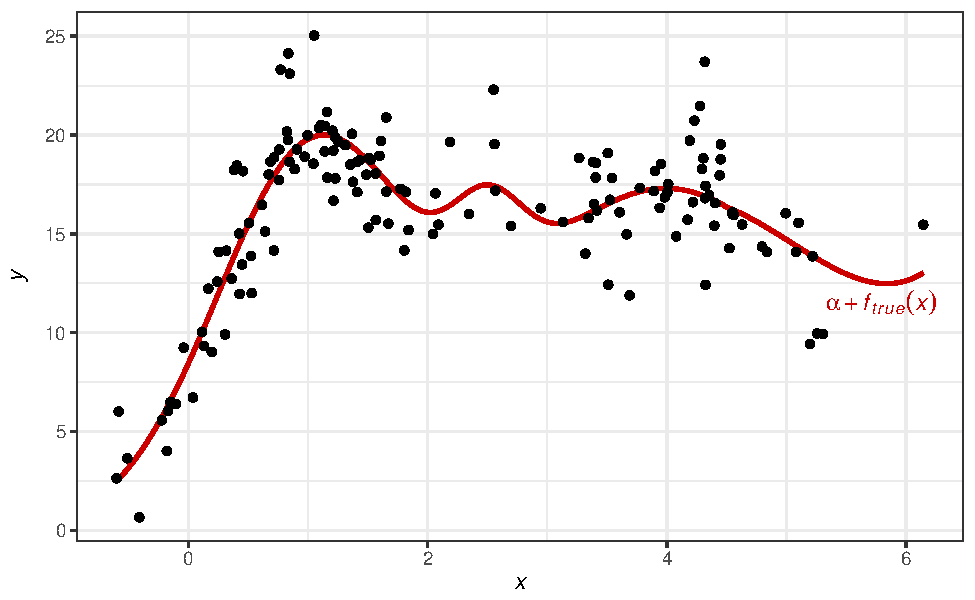
\includegraphics[width=0.8\textwidth]{figure/04-example_data}
  \caption{A plot of the sampled data points according to equation \cref{eq:examplesmoothingdata}, with the true regression function superimposed.}
  \label{fig:examplesmoothingdata}
\end{figure}

We attempt to estimate $f_\text{true}$ by a function $f$ belonging to the fBm-0.5 RKHS $\cF_\lambda$, with an I-prior on $f$.
There are two parameters that need to be estimated: the scale parameter $\lambda$ for the fBm-0.5 RKHS, and the error precision $\psi$.
These can be estimated using the maximum likelihood methods described above, namely by direct optimisation and the EM algorithm.
These two methods are implemented in the \pkg{iprior} package. 
A full Bayesian treatment is possible, and we use the \pkg{rstan} implementation of \proglang{Stan} to perform Hamiltonian Monte Carlo sampling of the posterior densities.
A vague prior choice for $\lambda$ and $\psi$ are prescribed, namely
\[
  \lambda,\psi \iid \N_+(0,100),
\]
where $\N_+(\mu,\sigma^2)$ represents the \emph{half-normal} distribution\footnote{The random variable $X \sim \N_+(\mu,\sigma^2)$ has the density $p(x) = \phi(x|\mu,\sigma^2)\ind(x \geq 0)$.}.
We have also set an improper prior density $p(\alpha) \propto \const$ for the intercept.
The advantage of HMC is that efficiency is not dictated by conjugacy, so there is freedom to choose any appropriate prior choice on the parameters.

\begin{table}[hbt]
\centering
\caption{Table comparing the estimated parameter values, (marginal) log-likelihood values, and also time taken for the three estimation methods.}
\label{tab:comparemethodsestimate}
\begin{tabular}{@{}lrrr@{}}
\toprule
               & Direct optimisation & EM algorithm & Hamiltonian MC          \\ \midrule
Intercept ($\alpha$)      & 16.1 (NA)           & 16.1 (NA)    & 16.1 (0.17)  \\
Scale ($\lambda$)      & 5.01 (1.23)         & 5.01 (1.26)  & 5.61 (1.42)     \\
Precision ($\psi$)         & 0.236 (0.03)        & 0.236 (0.03) & 0.237 (0.03)\\[0.5em]
Log density    & -339.7              & -339.7       & -341.1                  \\
Predictive RMSE & 0.574               & 0.575        & 0.582                   \\[0.5em]
Iterations     & 12                  & 266          & 2000                    \\
Time taken (s) & 0.96                & 3.65         & 232                     \\ \bottomrule
\end{tabular}
\end{table}

Table \ref{tab:comparemethodsestimate} tabulates the estimated parameter values, (marginal) log-likelihood values, and also time taken for the three estimation methods.
The three methods concur on the estimated parameter values, although the scale parameter has been estimated slightly differently, which is possibly attributed to the effect of the prior for $\lambda$.
The resulting log-likelihood value for the Bayesian method is lower than the ML methods, which also took the longest to compute.
Although the EM algorithm took longer than the direct optimisation method to compute, the time taken per iteration is significantly shorter than one Newton iteration.
%In this simple example, there were no numerical issues encountered with the direct optimisation method, but in more complex examples (see \hltodo{Section X}), instabilities could arise.


\section{Examples}
%\documentclass[a4paper,showframe,11pt]{report}\usepackage[]{graphicx}\usepackage[]{color}
%% maxwidth is the original width if it is less than linewidth
%% otherwise use linewidth (to make sure the graphics do not exceed the margin)
\makeatletter
\def\maxwidth{ %
  \ifdim\Gin@nat@width>\linewidth
    \linewidth
  \else
    \Gin@nat@width
  \fi
}
\makeatother

\definecolor{fgcolor}{rgb}{0.196, 0.196, 0.196}
\newcommand{\hlnum}[1]{\textcolor[rgb]{0.063,0.58,0.627}{#1}}%
\newcommand{\hlstr}[1]{\textcolor[rgb]{0.063,0.58,0.627}{#1}}%
\newcommand{\hlcom}[1]{\textcolor[rgb]{0.588,0.588,0.588}{#1}}%
\newcommand{\hlopt}[1]{\textcolor[rgb]{0.196,0.196,0.196}{#1}}%
\newcommand{\hlstd}[1]{\textcolor[rgb]{0.196,0.196,0.196}{#1}}%
\newcommand{\hlkwa}[1]{\textcolor[rgb]{0.231,0.416,0.784}{#1}}%
\newcommand{\hlkwb}[1]{\textcolor[rgb]{0.627,0,0.314}{#1}}%
\newcommand{\hlkwc}[1]{\textcolor[rgb]{0,0.631,0.314}{#1}}%
\newcommand{\hlkwd}[1]{\textcolor[rgb]{0.78,0.227,0.412}{#1}}%
\let\hlipl\hlkwb

\usepackage{framed}
\makeatletter
\newenvironment{kframe}{%
 \def\at@end@of@kframe{}%
 \ifinner\ifhmode%
  \def\at@end@of@kframe{\end{minipage}}%
  \begin{minipage}{\columnwidth}%
 \fi\fi%
 \def\FrameCommand##1{\hskip\@totalleftmargin \hskip-\fboxsep
 \colorbox{shadecolor}{##1}\hskip-\fboxsep
     % There is no \\@totalrightmargin, so:
     \hskip-\linewidth \hskip-\@totalleftmargin \hskip\columnwidth}%
 \MakeFramed {\advance\hsize-\width
   \@totalleftmargin\z@ \linewidth\hsize
   \@setminipage}}%
 {\par\unskip\endMakeFramed%
 \at@end@of@kframe}
\makeatother

\definecolor{shadecolor}{rgb}{.97, .97, .97}
\definecolor{messagecolor}{rgb}{0, 0, 0}
\definecolor{warningcolor}{rgb}{1, 0, 1}
\definecolor{errorcolor}{rgb}{1, 0, 0}
\newenvironment{knitrout}{}{} % an empty environment to be redefined in TeX

\usepackage{alltt}
\usepackage{standalone}
\standalonetrue
\ifstandalone
  \usepackage{../../haziq_thesis}
  \usepackage{../../haziq_maths}
  \usepackage{../../haziq_glossary}
  \addbibresource{../../bib/haziq.bib}
  \externaldocument{../01/.texpadtmp/introduction}
  \externaldocument{../02/.texpadtmp/chapter2}
  \externaldocument{../03/.texpadtmp/chapter3}
\fi




\IfFileExists{upquote.sty}{\usepackage{upquote}}{}
\begin{document}

We demonstrate the use of the \pkg{iprior} package with modelling a toy example from a simulated data set, as well as three other real-data examples.

\subsection[Using the Nystrom method]{Using the Nystr\"om method}

In this section, we investigate the use of the Nystr\"om method of approximating the kernel matrix in estimating I-prior models applied to a toy data set.
The data is obtained by randomly generating data points according to the true regression model
%
\begin{align*}
  \begin{gathered}
    y_i = \const + \, 0.35 \cdot \phi(x_i;1,0.8^2) + 0.65 \cdot \phi(x_i;4,1.5^2)
    + \ind[x_i > 4.5]\cdot e^{1.25(x_i-4.5)} + \epsilon_i \\
    \epsilon_i \iid \N(0, 0.9 ^ 2)
  \end{gathered}
\end{align*}
%
where $\phi(x;\mu,\sigma^2)$ represents the PDF of a normal distribution with mean $\mu$ and variance $\sigma^2$.
The features of this regression function are two large bumps at the centres of the mixed Gaussian PDFs, and also a small bump right after $x>4.5$ caused by the additional exponential function.
The true regression function goes to positive infinity as $x$ increases, and to zero as $x$ decreases.
2,000 $(x,y)$ points in the domain $x \in (-1, 5.5)$ have been generated by the built-in \code{gen_smooth()} function, which generates data from the regression model above\footnote{Random fluctuations have also been added to the $(x,y)$ coordinates.}.

\begin{knitrout}
\definecolor{shadecolor}{rgb}{1, 1, 1}\color{fgcolor}\begin{kframe}
\singlespacing\begin{alltt}
\hlstd{R> }\hlstd{dat} \hlkwb{<-} \hlkwd{gen_smooth}\hlstd{(}\hlkwc{n} \hlstd{=} \hlnum{2000}\hlstd{,} \hlkwc{xlim} \hlstd{=} \hlkwd{c}\hlstd{(}\hlopt{-}\hlnum{1}\hlstd{,} \hlnum{5.5}\hlstd{),} \hlkwc{seed} \hlstd{=} \hlnum{1}\hlstd{)}
\hlstd{R> }\hlkwd{head}\hlstd{(dat)}
\end{alltt}
\begin{verbatim}
##            y         X
## 1  0.6803514 -2.608953
## 2  3.6747031 -2.554039
## 3 -1.1563508 -2.381275
## 4  2.2657657 -2.280259
## 5  2.5398243 -2.214122
## 6  1.2929592 -2.170532
\end{verbatim}
\end{kframe}
\end{knitrout}

One could fit the regression model using all available data points, with an I-prior from the fBm-0.5 RKHS of functions as follows (note that the \code{silent} option is used to suppress the output from the \code{iprior()} function):

\begin{knitrout}
\definecolor{shadecolor}{rgb}{1, 1, 1}\color{fgcolor}\begin{kframe}
\singlespacing\begin{alltt}
\hlstd{R> }\hlstd{(mod.full} \hlkwb{<-} \hlkwd{iprior}\hlstd{(y} \hlopt{~} \hlstd{X, dat,} \hlkwc{kernel} \hlstd{=} \hlstr{"fbm"}\hlstd{,}
\hlstd{+  }                    \hlkwc{control} \hlstd{=} \hlkwd{list}\hlstd{(}\hlkwc{silent} \hlstd{=} \hlnum{TRUE}\hlstd{)))}
\end{alltt}
\begin{verbatim}
## Log-likelihood value: -4355.075 
## 
##  lambda     psi 
## 2.30244 0.23306
\end{verbatim}
\end{kframe}
\end{knitrout}

To implement the Nystr\"om method, the option \code{nystrom = 50} was added to the above function call, which uses 50 randomly selected data points for the Nystr\"om approximation.

\begin{knitrout}
\definecolor{shadecolor}{rgb}{1, 1, 1}\color{fgcolor}\begin{kframe}
\singlespacing\begin{alltt}
\hlstd{R> }\hlstd{(mod.nys} \hlkwb{<-} \hlkwd{iprior}\hlstd{(y} \hlopt{~} \hlstd{X, dat,} \hlkwc{kernel} \hlstd{=} \hlstr{"fbm"}\hlstd{,} \hlkwc{nystrom} \hlstd{=} \hlnum{50}\hlstd{,}
\hlstd{+  }                   \hlkwc{control} \hlstd{=} \hlkwd{list}\hlstd{(}\hlkwc{silent} \hlstd{=} \hlnum{TRUE}\hlstd{)))}
\end{alltt}
\begin{verbatim}
## Log-likelihood value: -1945.33 
## 
##  lambda     psi 
## 1.64833 0.13538
\end{verbatim}
\end{kframe}
\end{knitrout}

The hyperparameters estimated for both models are slightly different.
The log-likelihood is also different, but this is attributed to information loss due to the approximation procedure.
Nevertheless, we see from Figure \ref{fig:nystrom.plot} that the estimated regression functions are quite similar in both the full model and the approximated model.
The main difference is that the the Nystr\"om method was not able to extrapolate the right hand side of the plot well, because it turns out that there were no data points used from this region.
This can certainly be improved by using a more intelligent sampling scheme.
The full model took a little under 15 minutes to converge, while the Nystr\"om method took just seconds.
Storage savings is significantly higher with the Nystr\"om method as well.

\begin{knitrout}
\definecolor{shadecolor}{rgb}{1, 1, 1}\color{fgcolor}\begin{kframe}
\singlespacing\begin{alltt}
\hlstd{R> }\hlkwd{get_time}\hlstd{(mod.full);} \hlkwd{get_size}\hlstd{(mod.full,} \hlkwc{units} \hlstd{=} \hlstr{"MB"}\hlstd{)}
\end{alltt}
\begin{verbatim}
## 14.63474 mins
## 128.2 MB
\end{verbatim}
\begin{alltt}
\hlstd{R> }\hlkwd{get_time}\hlstd{(mod.nys);} \hlkwd{get_size}\hlstd{(mod.nys)}
\end{alltt}
\begin{verbatim}
## 1.324355 secs
## 965.2 kB
\end{verbatim}
\end{kframe}
\end{knitrout}

\begin{knitrout}
\definecolor{shadecolor}{rgb}{1, 1, 1}\color{fgcolor}\begin{kframe}
\singlespacing\end{kframe}\begin{figure}

{\centering 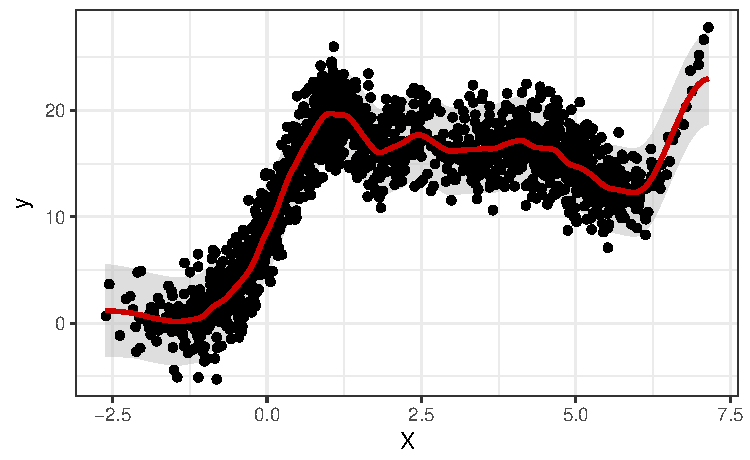
\includegraphics[width=7.7cm,height=4.8cm]{figure/04-nystrom_plot-1} 
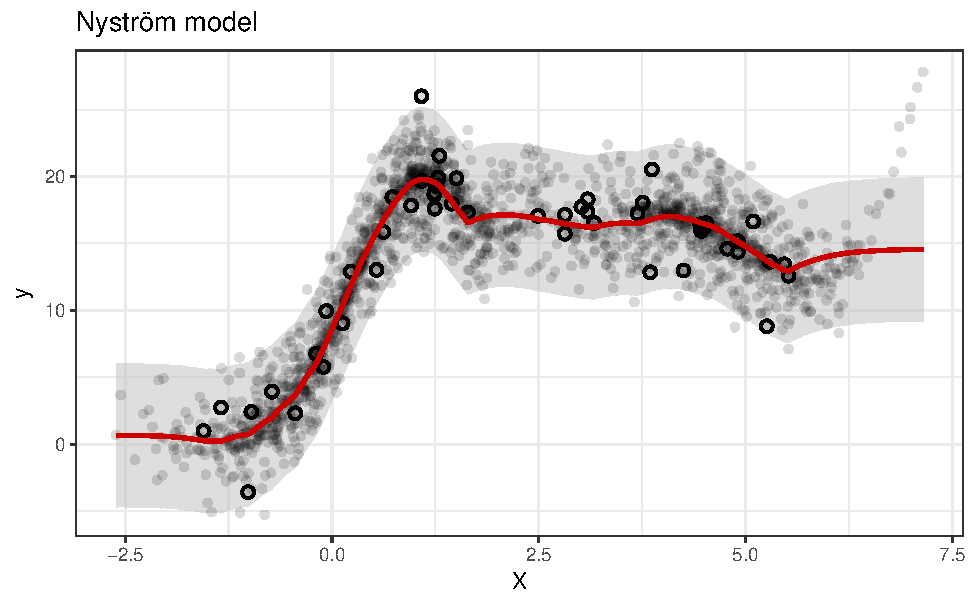
\includegraphics[width=7.7cm,height=4.8cm]{figure/04-nystrom_plot-2} 

}

\caption[Plot of predicted regression function for the full model (left) and the Nystr\"om approximated method (right)]{Plot of predicted regression function for the full model (left) and the Nystr\"om approximated method (right). For the Nystr\"om plot, the data points that were active are shown by circles with bold outlines.}\label{fig:nystrom.plot}
\end{figure}


\end{knitrout}

\subsection{Random effects models}

In this section, a comparison between a standard random effects model and the I-prior approach for estimating varying intercept and slopes model is illustrated.
The example concerns control data\footnotemark\ from several runs of radioimmunoassays (RIA) for the protein insulin-like growth factor (IGF-I) (explained in further detail in \citealt{davidian1995nonlinear}, Section 3.2.1).
RIA is a in vitro assay technique which is used to measure concentration of antigens---in our case, the IGF-I proteins.
When an RIA is run, control samples at known concentrations obtained from a particular lot are included for the purpose of assay quality control.
It is expected that the concentration of the control material remains stable as the machine is used, up to a maximum of about 50 days, at which point  control samples from a new batch is used to avoid degradation in assay performance.

\begin{knitrout}
\definecolor{shadecolor}{rgb}{1, 1, 1}\color{fgcolor}\begin{kframe}
\singlespacing\begin{alltt}
\hlstd{R> }\hlkwd{data}\hlstd{(IGF,} \hlkwc{package} \hlstd{=} \hlstr{"nlme"}\hlstd{)}
\hlstd{R> }\hlkwd{head}\hlstd{(IGF)}
\end{alltt}
\begin{verbatim}
## Grouped Data: conc ~ age | Lot
##   Lot age conc
## 1   1   7 4.90
## 2   1   7 5.68
## 3   1   8 5.32
## 4   1   8 5.50
## 5   1  13 4.94
## 6   1  13 5.19
\end{verbatim}
\end{kframe}
\end{knitrout}

\footnotetext{This data is available in the \proglang{R} package \pkg{nlme} \citep{nlme}.}

The data consists of IGF-I concentrations (\code{conc}) from control samples from 10 different lots measured at differing \code{age}s of the lot.
The data were collected with the aim of identifying possible trends in control values \code{conc} with \code{age}, ultimately investigating whether or not the usage protocol of maximum sample age of 50 days is justified.
\cite{pinheiro2000mixed} remarks that this is not considered a longitudinal problem because different samples were used at each measurement.

We shall  model the IGF data set using the I-prior methodology using the regression function
%
\[
  f(\texttt{age}, \texttt{Lot}) = f_1(\texttt{age}) + f_2(\texttt{Lot}) + f_{12}(\texttt{age}, \texttt{Lot})
\]
%
where $f_1$ lies in the linear RKHS $\cF_1$, $f_2$ in the Pearson RKHS $\cF_2$ and $f_{12}$ in the tensor product space $\cF_{12} = \cF_1 \otimes \cF_2$.
The regression function $f$ then lies in the RKHS $\cF = \cF_1 \oplus \cF_2 \oplus \cF_{12}$ with kernel equal to the sum of the kernels from each of the RKHSs\footnote{This is often known as the functional ANOVA decomposition.}.
The explanation here is that the \code{conc} levels are assumed to be related to both \code{age} and \code{Lot}, and in particular, the contribution of \code{age} on \code{conc} varies with each individual \code{Lot}.
This gives the intended effect of a linear mixed-effects model, which is thought to be suitable in this case, in order to account for within-lot and between-lot variability.
We first fit the model using the \pkg{iprior} package, and then compare the results with the standard random effects model using \code{lme4::lmer()}.
The command to fit the I-prior model using the EM algorithm is

\begin{knitrout}
\definecolor{shadecolor}{rgb}{1, 1, 1}\color{fgcolor}\begin{kframe}
\singlespacing\begin{alltt}
\hlstd{R> }\hlstd{mod.iprior} \hlkwb{<-} \hlkwd{iprior}\hlstd{(conc} \hlopt{~} \hlstd{age} \hlopt{*} \hlstd{Lot, IGF,} \hlkwc{method} \hlstd{=} \hlstr{"em"}\hlstd{)}
\end{alltt}
\begin{verbatim}
## ========================================
## Converged after 57 iterations.
\end{verbatim}
\begin{alltt}
\hlstd{R> }\hlkwd{summary}\hlstd{(mod.iprior)}
\end{alltt}
\begin{verbatim}
## Call:
## iprior(formula = conc ~ age * Lot, data = IGF, method = "em")
## 
## RKHS used:
## Linear (age)
## Pearson (Lot)
## 
## Residuals:
##    Min. 1st Qu.  Median 3rd Qu.    Max. 
## -4.4889 -0.3798 -0.0090  0.2563  4.3973 
## 
## Hyperparameters:
##           Estimate   S.E.      z P[|Z>z|]    
## lambda[1]   0.0000 0.0002 -0.004    0.997    
## lambda[2]   0.0007 0.0030  0.238    0.812    
## psi         1.4576 0.1366 10.672   <2e-16 ***
## ---
## Signif. codes:  0 '***' 0.001 '**' 0.01 '*' 0.05 '.' 0.1 ' ' 1
## 
## Closed-form EM algorithm. Iterations: 57/100 
## Converged to within 1e-08 tolerance. Time taken: 3.043089 secs
## Log-likelihood value: -291.9033 
## RMSE of prediction: 0.8273639 (Training)
\end{verbatim}
\end{kframe}
\end{knitrout}
\begin{knitrout}
\definecolor{shadecolor}{rgb}{1, 1, 1}\color{fgcolor}\begin{kframe}
\singlespacing\end{kframe}\begin{figure}

{\centering 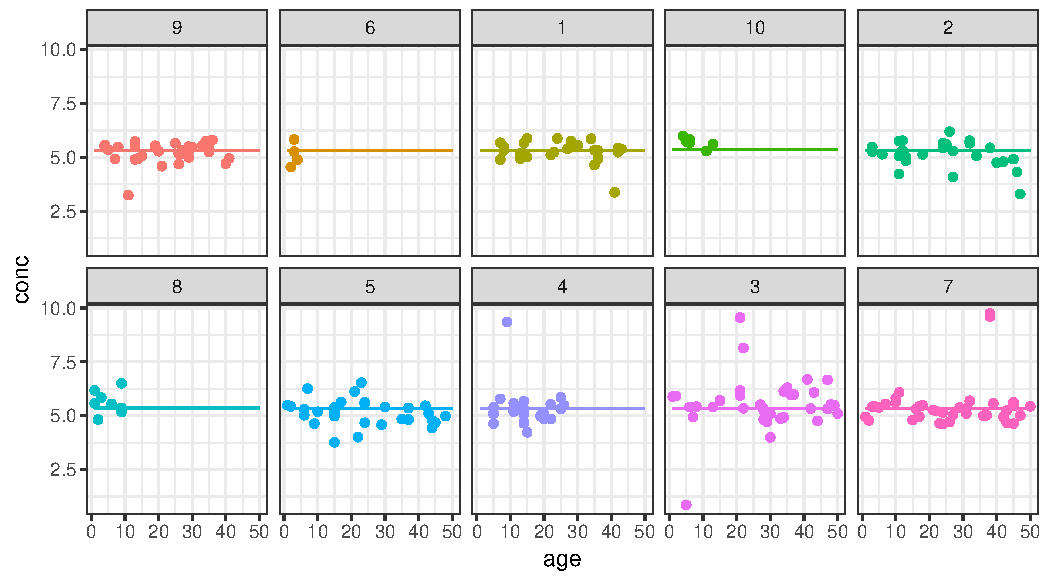
\includegraphics[width=\maxwidth]{figure/04-IGF_mod_iprior_plot-1} 

}

\caption[Plot of fitted regression line for the I-prior model on the IGF data set, separated into each of the 10 lots]{Plot of fitted regression line for the I-prior model on the IGF data set, separated into each of the 10 lots.}\label{fig:IGF.mod.iprior.plot}
\end{figure}


\end{knitrout}

To make inference on the covariates, we look at the scale parameters \code{lambda}.
We see that both scale parameters for \code{age} and \code{Lot} are close to zero, and a test of significance is not able to reject the hypothesis that these parameters are indeed null.
We conclude that neither \code{age} nor \code{Lot} has a linear effect on the \code{conc} levels.
The plot of the fitted regression line in Figure \ref{fig:IGF.mod.iprior.plot} does show an almost horizontal line for each \code{Lot}.
% Another way of looking at this problem is to compare the fitted model with a constant model, i.e., a model with only the intercept fitted.
% This model is able to be fitted by constraining and the \code{lambda} parameters to zero, as follows:

% <IGF.mod.iprior.const, cache = TRUE>>=
% @

% We then perform a log-likelihood ratio test to compare the two models.
% The test statistic yields a value of round(D) which follows an asymptotic $\chi^2$ distribution with two degrees of freedom (three parameters estimated in the original model, and only one in the constant model).

%\newpage
The standard random effects model, as explored by \cite{davidian1995nonlinear} and \cite{pinheiro2000mixed}, is
%
\begin{align*}
  \begin{gathered}
    \texttt{conc}_{ij} = \beta_{0j} + \beta_{1j}\texttt{age}_{ij} + \epsilon_{ij} \\
    \begin{pmatrix}
      \beta_{0j} \\
      \beta_{1j} \\
    \end{pmatrix}
    \sim \N \left(
      \begin{pmatrix}
        \beta_{0} \\
        \beta_{1} \\
      \end{pmatrix},
      \begin{pmatrix}
        \sigma_{0}^2 & \sigma_{01} \\
        \sigma_{01}  & \sigma_1^2 \\
      \end{pmatrix}
    \right) \\
    \epsilon_{ij} \sim \N(0, \sigma^2) \\
  \end{gathered}
\end{align*}
%
for $i=1,\dots,n_j$ and the index $j$ representing the 10 \code{Lots}.
Fitting this model using \code{lmer}, we can test for the significance of the fixed effect $\beta_0$, for which we find that it is not ($p$-value = 0.616), and arrive at the same conclusion as in the I-prior model.
However, we notice that the package reports a perfect negative correlation between the random effects, $\sigma_{01}$.
This indicates a potential numerical issue when fitting the model---a value of exactly $-1$, $0$ or $1$ is typically imposed by the package to force through estimation in the event of non-positive definite covariance matrices arising.
We can inspect the eigenvalues of the covariance matrix for the random effects to check that they are indeed non-positive definite.

\begin{knitrout}
\definecolor{shadecolor}{rgb}{1, 1, 1}\color{fgcolor}\begin{kframe}
\singlespacing\begin{alltt}
\hlstd{R> }\hlstd{(mod.lmer} \hlkwb{<-} \hlkwd{lmer}\hlstd{(conc} \hlopt{~} \hlstd{age} \hlopt{+} \hlstd{(age} \hlopt{|} \hlstd{Lot), IGF))}
\end{alltt}
\begin{verbatim}
## Linear mixed model fit by REML ['lmerMod']
## Formula: conc ~ age + (age | Lot)
##    Data: IGF
## REML criterion at convergence: 594.3662
## Random effects:
##  Groups   Name        Std.Dev. Corr 
##  Lot      (Intercept) 0.082507      
##           age         0.008092 -1.00
##  Residual             0.820628      
## Number of obs: 237, groups:  Lot, 10
## Fixed Effects:
## (Intercept)          age  
##    5.374974    -0.002535
\end{verbatim}
\begin{alltt}
\hlstd{R> }\hlkwd{eigen}\hlstd{(}\hlkwd{VarCorr}\hlstd{(mod.lmer)}\hlopt{$}\hlstd{Lot)}
\end{alltt}
\begin{verbatim}
## eigen() decomposition
## $values
## [1]  6.872939e-03 -1.355253e-20
## 
## $vectors
##             [,1]        [,2]
## [1,] -0.99522490 -0.09760839
## [2,]  0.09760839 -0.99522490
\end{verbatim}
\end{kframe}
\end{knitrout}

\begin{knitrout}
\definecolor{shadecolor}{rgb}{1, 1, 1}\color{fgcolor}\begin{kframe}
\singlespacing\end{kframe}\begin{figure}[t]

{\centering 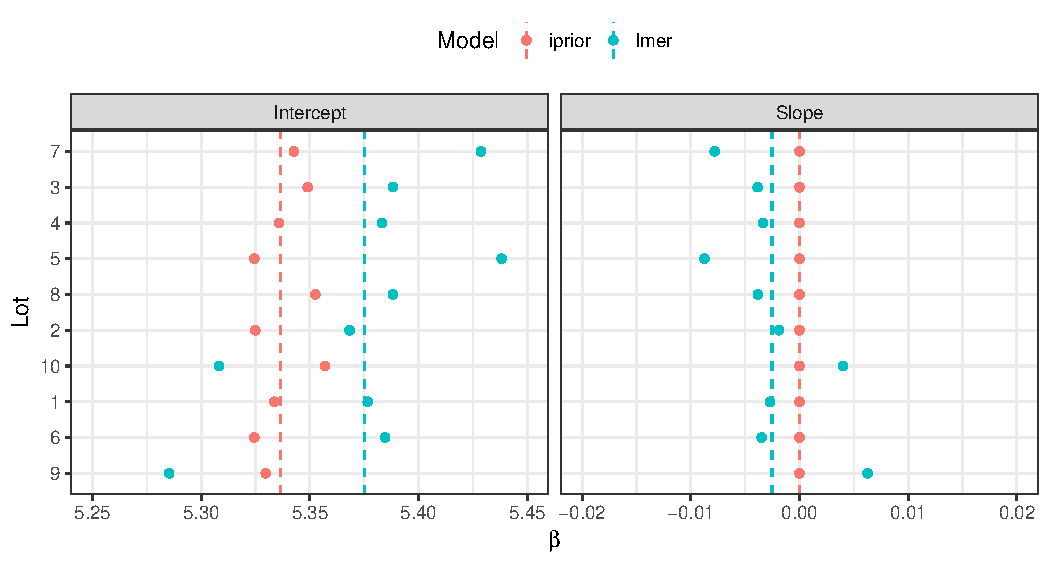
\includegraphics[width=\maxwidth]{figure/04-IGF_plot_beta-1} 

}

\caption[A comparison of the estimates for random intercepts and slopes (denoted as points) using the I-prior model and the standard random effects model]{A comparison of the estimates for random intercepts and slopes (denoted as points) using the I-prior model and the standard random effects model. The dashed vertical lines indicate the fixed effect values.}\label{fig:IGF.plot.beta}
\end{figure}


\end{knitrout}

\begin{table}[b!]
\centering
\begin{tabular}{lrr}
\toprule
Parameter     & \texttt{iprior} & \texttt{lmer} \\
\midrule
$\sigma_0$    & 0.012 & 0.083 \\
$\sigma_1$    & 0.000 & 0.008 \\
$\rho_{01}$   & 0.690& -1.000 \\
\bottomrule
\end{tabular}
\caption{A comparison of the estimates for the covariance matrix of the random effects using the I-prior model and the standard random effects model.}
\label{tab:igf}
\end{table}

Degenerate covariance matrices often occur in models with a large number of random coefficients.
These are typically solved by setting restrictions which then avoids overparameterising the model.
One advantage of the I-prior method for varying intercept/slopes model is that the positive-definiteness is automatically taken care of.
Furthermore, I-prior models typically require less number of parameters to fit a similar varying intercept/slopes model -- in the above example, the I-prior model estimated only three parameters, while the standard random effects model estimated a total of six parameters.

It is also possible to ``recover'' the estimates of the standard random effects model from the I-prior model, albeit in a slighly manual fashion.
Denote by $f^j$ the individual linear regression lines for each of the $j=1,\dots,10$ \code{Lots}.
Then, each of these $f^j$ has a slope and intercept for which we can estimate from the fitted values $\hat f^j(x_{ij})$, $i=1,\dots,n_j$.
This would give us the estimate of the posterior mean of the random intercepts and slopes; these would typically be obtained using empirical-Bayes methods in the case of the standard random effects model.

Furthermore, $\sigma_0^2$ and $\sigma_1^2$ gives a measure of variability of the intercepts and slopes of the different groups, and this can be calculated from the estimates of the random intercepts and slopes.
In the same spirit, $\rho_{01} = \sigma_{01} / (\sigma_0 \sigma_1)$, which is the correlation between the random intercept and slope, can be similarly calculated.
Finally, the fixed effects can be estimated from the intercept and slope of the best fit line running through the I-prior estimated \code{conc} values.
The intuition for this is that the fixed effects are essentially the ordinary least squares (OLS) of a linear model if the groupings are disregarded.
Figure \ref{fig:IGF.plot.beta} illustrates the differences in the estimates for the random coefficients, while Table \ref{tab:igf} illustrates the differences in the estimates for the covariance matrix.
Minor differences do exist, with the most noticeable one being that the slopes in the I-prior model are categorically estimated as zero, and the sign of the correlation $\rho_{01}$ being opposite in both models.
Even so, the conclusions from both models are similar.

\subsection{Longitudinal data analysis}
\label{sec:cows}

We consider a balanced longitudinal data set consisting of weights in kilograms of 60 cows, 30 of which were randomly assigned to treatment group A, and the remaining 30 to treatment group B.
The animals were weighed 11 times over a 133-day period; the first 10 measurements for each animal were made at two-week intervals and the last measurement was made one week later.
This experiment was reported by \cite{kenward1987method}, and the data set is included as part of the package \pkg{jmcm} \citep{jmcm} in \proglang{R}.
The variable names have been renamed for convenience.

\begin{knitrout}
\definecolor{shadecolor}{rgb}{1, 1, 1}\color{fgcolor}\begin{kframe}
\singlespacing\begin{alltt}
\hlstd{R> }\hlkwd{data}\hlstd{(cattle,} \hlkwc{package} \hlstd{=} \hlstr{"jmcm"}\hlstd{)}
\hlstd{R> }\hlkwd{names}\hlstd{(cattle)} \hlkwb{<-} \hlkwd{c}\hlstd{(}\hlstr{"id"}\hlstd{,} \hlstr{"time"}\hlstd{,} \hlstr{"group"}\hlstd{,} \hlstr{"weight"}\hlstd{)}
\hlstd{R> }\hlstd{cattle}\hlopt{$}\hlstd{id} \hlkwb{<-} \hlkwd{as.factor}\hlstd{(cattle}\hlopt{$}\hlstd{id)}  \hlcom{# convert to factors}
\hlstd{R> }\hlkwd{str}\hlstd{(cattle)}
\end{alltt}
\begin{verbatim}
## 'data.frame':	660 obs. of  4 variables:
##  $ id    : Factor w/ 60 levels "1","2","3","4",..: 1 1 1 1 1 1 1 1 1..
##  $ time  : num  0 14 28 42 56 70 84 98 112 126 ...
##  $ group : Factor w/ 2 levels "A","B": 1 1 1 1 1 1 1 1 1 1 ...
##  $ weight: int  233 224 245 258 271 287 287 287 290 293 ...
\end{verbatim}
\end{kframe}
\end{knitrout}

The response variable of interest are the \code{weight} growth curves, and the aim is to investigate whether a treatment effect is present.
The usual approach to analyse a longitudinal data set such as this one is to assume that the observed growth curves are realizations of a Gaussian process.
For example, \cite{kenward1987method} assumed a so-called ante-dependence structure of order $k$, which assumes an observation depends on the previous $k$ observations, but given these, is independent of any preceeding observations.

Using the I-prior, it is not necessary to assume the growth curves were drawn randomly.
Instead, it suffices to assume that they lie in an appropriate function class.
For this example, we assume that the function class is the fBm RKHS, i.e., we assume a smooth effect of time on weight.
The growth curves form a multidimensional (or functional) response equivalent to a ``wide'' format of representing repeated measures data. In our analysis using the \pkg{iprior} package, we used the ``long'' format and thus our (unidimensional) sample size $n$ is equal to $60$ cows $\times$ $11$ repeated measurements.
We also have two covariates potentially influencing growth, namely the cow subject \code{id} and also treatment \code{group}. The regression model can then be thought of as
%
\begin{align*}
  \begin{gathered}
    \text{\code{weight}} = \alpha + f(\text{\code{id}}, \, \text{\code{group}}, \, \text{\code{time}}) + \epsilon \\
    \epsilon \sim \N(0, \psi^{-1}).
  \end{gathered}
\end{align*}
%
\begin{table}[t!]
\centering
\begin{tabular}{lp{6cm}l}
\toprule
Model & Explanation & Formula (\verb@weight ~ ...@) \\
\midrule
1     & Growth does not vary with treatment nor among cows
&\verb@time@ \\
2     & Growth varies among cows only
&\verb@id * time@ \\
3     & Growth varies with treatment only
&\verb@group * time@ \\
4     & Growth varies with treatment and among cows
&\verb@id * time + group * time@ \\
5     & Growth varies with treatment and among cows, with an interaction effect between treatment and cows
&\verb@id * group * time@ \\
\bottomrule
\end{tabular}
\caption{A brief description of the five models fitted using I-priors.}
\label{tab:cowmodel}
\end{table}

\vspace{-1em}
We assume iid errors, and in addition to a smooth effect of \code{time}, we further assume a nominal effect of both cow \code{id} and treatment \code{group} using the Pearson RKHS.
In the \pkg{iprior} package, factor type objects are treated with the Pearson kernel automatically, and the only \code{model} option we need to specify is the \code{kernel = "fbm"} option for the \code{time} variable.
We have opted not to estimate the Hurst coefficient in the interest of computational time, and instead left it at the default value of 0.5.
Table \ref{tab:cowmodel} explains the five models we have fitted.

The simplest model fitted was one in which the growth curves do not depend on the treatment effect or individual cows.
We then added treatment effect and the cow \code{id} as covariates, separately first and then together at once.
We also assumed that both of these covariates are time-varying, and hence added also the interaction between these covariates and the \code{time} variable.
The final model was one in which an interaction between treatment effect and individual cows was assumed, which varied over time.

All models were fitted using the \code{mixed} estimation method.
Compared to the EM algorithm alone, we found that the combination of direct optimisation with the EM algorithm in the \code{mixed} routine fits the model about six times faster for this data set due to slow convergence of EM algorithm.
Here is the code and output for fitting the first model:

\begin{knitrout}
\definecolor{shadecolor}{rgb}{1, 1, 1}\color{fgcolor}\begin{kframe}
\singlespacing\begin{alltt}
\hlstd{R> }\hlcom{# Model 1: weight ~ f(time)}
\hlstd{R> }\hlstd{(mod1} \hlkwb{<-} \hlkwd{iprior}\hlstd{(weight} \hlopt{~} \hlstd{time, cattle,} \hlkwc{kernel} \hlstd{=} \hlstr{"fbm"}\hlstd{,} \hlkwc{method} \hlstd{=} \hlstr{"mixed"}\hlstd{))}
\end{alltt}
\begin{verbatim}
## Running 5 initial EM iterations
## ======================================================================
## Now switching to direct optimisation
## final  value 1394.615060 
## converged
## Log-likelihood value: -2789.231 
## 
##  lambda     psi 
## 0.83656 0.00375
\end{verbatim}
\end{kframe}
\end{knitrout}


\newcolumntype{R}[1]{>{\raggedleft\arraybackslash}p{#1}}
\begin{table}[t!]
\centering
\begin{tabular}{rp{4.9cm}R{2.3cm}R{1.9cm}R{2.2cm}}
\toprule
{\small Model}
& {\small{Formula \newline (}\verb@weight ~ ...@{)}}
& {\small{Log-likelihood}}
& {\small{Error S.D.}}
& {\small{Number of parameters}}  \\
\midrule
1 & \code{time}
& -2789.23
& 16.33
& 1 \\
2 & \code{id * time}
& -2789.20
& 16.32
& 2 \\
3 & \code{group * time}
& -2295.16
& 3.68
& 2 \\
4 & \code{id * time + group * time}
& -2787.03
& 15.91
& 3 \\
5 & \code{id * group * time}
& -2787.03
& 15.91
& 3 \\
\bottomrule
\end{tabular}
\caption{Summary of the five I-prior models fitted to the cow data set.}
\label{tab:cowresults}
\end{table}

\begin{knitrout}
\definecolor{shadecolor}{rgb}{1, 1, 1}\color{fgcolor}\begin{kframe}
\singlespacing\end{kframe}\begin{figure}[h]

{\centering 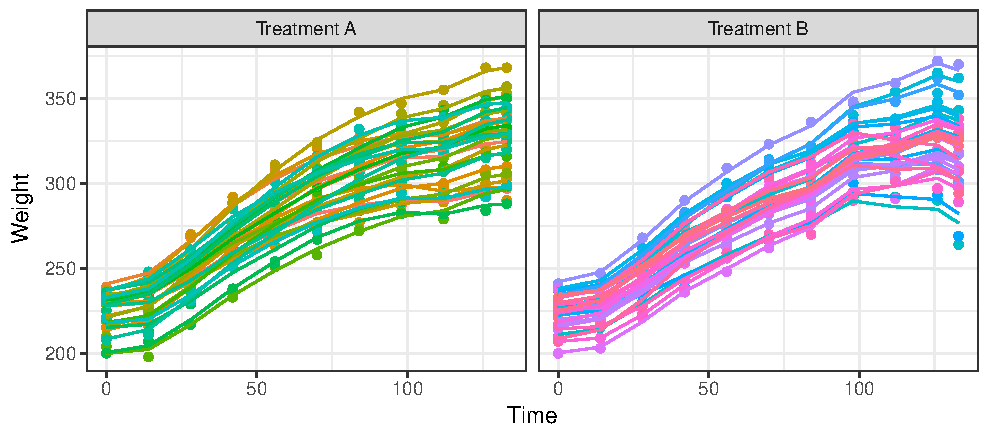
\includegraphics[width=\maxwidth]{figure/04-cows_plot-1} 

}

\caption[A plot of the I-prior fitted regression curves from Model 5]{A plot of the I-prior fitted regression curves from Model 5. In this model, growth curves differ among cows and by treatment effect (with an interaction between cows and treatment effect), thus producing these 60 individual lines, one for each cow, split between their respective treatment groups (A or B).}\label{fig:cows.plot}
\end{figure}


\end{knitrout}

The results of the model fit are summarised in Table \ref{tab:cowresults}. We can test for a treatment effect by testing Model 4 against the alternative that Model 2 is true.
The log-likelihood ratio test statistic is
$D = -2(-2789.20 - (-2787.03)) = 4.35$ which has an asymptotic chi-squared distribution with $3 - 2 = 1$ degree of freedom.
The $p$-value for this likelihood ratio test is less than $10^{-6}$, so we conclude that Model 4 is significantly better than Model 2.

We can next investigate whether the treatment effect differs among cows by comparing Model 5 against Model 4.
As these models have the same number of parameters, we can simply choose the one with the higher likelihood, which is Model 5.
We conclude that treatment does indeed have an effect on growth, and that the treatment effect differs among cows.
A plot of the fitted regression curves onto the cow data set is shown in Figure \ref{fig:cows.plot}.

\subsection{Regression with a functional covariate}

We illustrate the prediction of a real valued response with a functional covariate using a widely analysed data set for quality control in the food industry.
The data\footnotemark\ contain samples of spectrometric curve of absorbances of 215 pieces of finely chopped meat, along with their water, fat and protein content.
These data are recorded on a Tecator Infratec Food and Feed Analyzer working in the wavelength range 850--1050 nm by the Near Infrared Transmission (NIT) principle.
Absorption data has not been measured continuously, but instead 100 distinct wavelengths were obtained. Figure \ref{fig:tecator.data} shows a sample of 10 such spectrometric curves.

\footnotetext{
Obtained from Tecator (see \url{http://lib.stat.cmu.edu/datasets/tecator} for details).
We used the version made available in the dataframe \code{tecator} from the \proglang{R} package \pkg{caret} \citep{caret}.
}

\begin{knitrout}
\definecolor{shadecolor}{rgb}{1, 1, 1}\color{fgcolor}\begin{kframe}
\singlespacing\end{kframe}\begin{figure}

{\centering 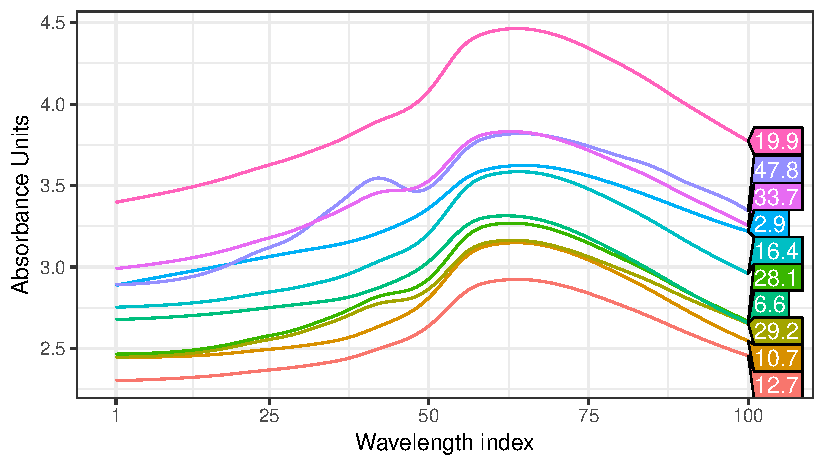
\includegraphics[width=12cm]{figure/04-tecator_data-1} 

}

\caption[Sample of spectrometric curves used to predict fat content of meat]{Sample of spectrometric curves used to predict fat content of meat. For each meat sample the data consists of a 100 channel spectrum of absorbances and the contents of moisture, fat (numbers shown in boxes) and protein measured in percent. The absorbance is $-\log 10$ of the transmittance measured by the spectrometer. The three contents, measured in percent, are determined by analytic chemistry.}\label{fig:tecator.data}
\end{figure}


\end{knitrout}

For our analyses and many others' in the literature, the first 172 observations in the data set are used as a training sample for model fitting, and the remaining 43 observations as a test sample to evaluate the predictive performance of the fitted model.
The focus here is to use the \pkg{iprior} package to fit several I-prior models to the Tecator data set, and calculate out-of-sample predictive error rates.
We compare the predictive performance of I-prior models against Gaussian process regression and the many other different methods applied on this data set.
These methods include neural networks \citep{thodberg1996review}, kernel smoothing \citep{ferraty2006nonparametric}, single and multiple index functional regression models \citep{chen2011single}, sliced inverse regression (SIR) and sliced average variance estimation (SAVE), multivariate adaptive regression splines (MARS), partial least squares (PLS), and functional additive model with and without component selection (FAM \& CSEFAM).
An analysis of this data set using the SIR and SAVE methods were conducted by  \cite{lian2014series}, while the MARS, PLS and (CSE)FAM methods were studied by \cite{zhu2014structured}.
Table \ref{tab:tecator} tabulates the results of all of these methods from the various references.

Assuming a regression model as in \eqref{eq:linmod}, we would like to model the \code{fat} content $y_i$ using the spectral curves $x_i$.
Let $x_i(t)$ denote the absorbance for wavelength $t = 1,\dots,100$.
From Figure \ref{fig:tecator.data}, it appears that the curves are smooth enough to be differentiable, and therefore it is reasonable to assume that they lie in the Sobolev-Hilbert space as discussed in Section \ref{sec:sobolevhilbert}.
We take first differences of the 100-dimensional matrix, which leaves us with the 99-dimensional covariate saved in the object named \code{absorp}.
The \code{fat} and \code{absorp} data have been split into \code{*.train} and \code{*.test} samples, as mentioned earlier.
Our first modelling attempt is to fit a linear effect by regressing the responses \code{fat.train} against a single high-dimensional covariate \code{absorp.train} using the linear RKHS and the direct optimisation method.

\begin{knitrout}
\definecolor{shadecolor}{rgb}{1, 1, 1}\color{fgcolor}\begin{kframe}
\singlespacing\begin{alltt}
\hlstd{R> }\hlcom{# Model 1: Canonical RKHS (linear)}
\hlstd{R> }\hlstd{(mod1} \hlkwb{<-} \hlkwd{iprior}\hlstd{(}\hlkwc{y} \hlstd{= fat.train, absorp.train))}
\end{alltt}
\begin{verbatim}
## iter   10 value 222.653144
## final  value 222.642108 
## converged
## Log-likelihood value: -445.2844 
## 
##     lambda        psi 
## 4576.86595    0.11576
\end{verbatim}
\end{kframe}
\end{knitrout}

Our second and third model uses polynomial RKHSs of degrees two and three, which allows us to model quadratic and cubic terms of the spectral curves respectively.
We also opted to estimate a suitable offset parameter, and this is called to \code{iprior()} with the option \code{est.offset = TRUE}.
Each of the two models has a single scale parameter, an offset parameter, and an error precision to be estimated.
The direct optimisation method has been used, and while both models converged regularly, it was noticed that there were multiple local optima that hindered the estimation (output omitted).

\begin{knitrout}
\definecolor{shadecolor}{rgb}{1, 1, 1}\color{fgcolor}\begin{kframe}
\singlespacing\begin{alltt}
\hlstd{R> }\hlcom{# Model 2: Polynomial RKHS (quadratic)}
\hlstd{R> }\hlstd{mod2} \hlkwb{<-} \hlkwd{iprior}\hlstd{(}\hlkwc{y} \hlstd{= fat.train, absorp.train,} \hlkwc{kernel} \hlstd{=} \hlstr{"poly2"}\hlstd{,}
\hlstd{+  }               \hlkwc{est.offset} \hlstd{=} \hlnum{TRUE}\hlstd{)}
\hlstd{R> }\hlcom{# Model 3: Polynomial RKHS (cubic)}
\hlstd{R> }\hlstd{mod3} \hlkwb{<-} \hlkwd{iprior}\hlstd{(}\hlkwc{y} \hlstd{= fat.train, absorp.train,} \hlkwc{kernel} \hlstd{=} \hlstr{"poly3"}\hlstd{,}
\hlstd{+  }               \hlkwc{est.offset} \hlstd{=} \hlnum{TRUE}\hlstd{)}
\end{alltt}
\end{kframe}
\end{knitrout}

Next, we attempt to fit a smooth dependence of fat content on the spectrometric curves using the fBm RKHS.
By default, the Hurst coefficient for the fBm RKHS is set to be 0.5.
However, with the option \code{est.hurst = TRUE}, the Hurst coefficient is included in the estimation procedure.
We fit models with both a fixed value for Hurst (at 0.5) and an estimated value for Hurst.
For both of these models, we encountered numerical issues when using the direct optimisation method.
%The L-BFGS algorithm kept on pulling the hyperparameter towards extremely high values, which in turn made the log-likelihood value greater than the machine's largest normalised floating-point number (\code{.Machine$double.xmax = 1.797693e+308}).
Investigating further, it seems that estimates at these large values give poor training and test error rates, though likelihood values here are high (local optima).
To get around this issue, we used the EM algorithm to estimate the fixed Hurst model, and the \code{mixed} method for the estimated Hurst model.
For both models, the \code{stop.crit} was relaxed and set to \code{1e-3} for quicker convergence, though this did not affect the predictive abilities compared to a more stringent \code{stop.crit}.

\begin{knitrout}
\definecolor{shadecolor}{rgb}{1, 1, 1}\color{fgcolor}\begin{kframe}
\singlespacing\begin{alltt}
\hlstd{R> }\hlcom{# Model 4: fBm RKHS (default Hurst = 0.5)}
\hlstd{R> }\hlstd{(mod4} \hlkwb{<-} \hlkwd{iprior}\hlstd{(}\hlkwc{y} \hlstd{= fat.train, absorp.train,} \hlkwc{kernel} \hlstd{=} \hlstr{"fbm"}\hlstd{,}
\hlstd{+  }                \hlkwc{method} \hlstd{=} \hlstr{"em"}\hlstd{,} \hlkwc{control} \hlstd{=} \hlkwd{list}\hlstd{(}\hlkwc{stop.crit} \hlstd{=} \hlnum{1e-3}\hlstd{)))}
\end{alltt}
\begin{verbatim}
## ==============================================
## Converged after 65 iterations.
## Log-likelihood value: -204.4592 
## 
##     lambda        psi 
##    3.24112 1869.32897
\end{verbatim}
\end{kframe}
\end{knitrout}
\begin{knitrout}
\definecolor{shadecolor}{rgb}{1, 1, 1}\color{fgcolor}\begin{kframe}
\singlespacing\begin{alltt}
\hlstd{R> }\hlcom{# Model 5: fBm RKHS (estimate Hurst)}
\hlstd{R> }\hlstd{(mod5} \hlkwb{<-} \hlkwd{iprior}\hlstd{(fat.train, absorp.train,} \hlkwc{kernel} \hlstd{=} \hlstr{"fbm"}\hlstd{,} \hlkwc{method} \hlstd{=} \hlstr{"mixed"}\hlstd{,}
\hlstd{+  }                \hlkwc{est.hurst} \hlstd{=} \hlnum{TRUE}\hlstd{,} \hlkwc{control} \hlstd{=} \hlkwd{list}\hlstd{(}\hlkwc{stop.crit} \hlstd{=} \hlnum{1e-3}\hlstd{)))}
\end{alltt}
\begin{verbatim}
## Running 5 initial EM iterations
## ======================================================================
## Now switching to direct optimisation
## iter   10 value 115.648462
## final  value 115.645800 
## converged
## Log-likelihood value: -231.2923 
## 
##    lambda     hurst       psi 
## 204.97184   0.70382   9.96498
\end{verbatim}
\end{kframe}
\end{knitrout}

Finally, we fit an I-prior model using the SE RKHS with lengthscale estimated.
Here we illustrate the use of the \code{restarts} option, in which the model is fitted repeatedly from different starting points.
In this case, eight random initial parameter values were used and these jobs were parallelised across the eight available cores of the machine.
The additional \code{par.maxit} option in the \code{control} list is an option for the maximum number of iterations that each parallel job should do.
We have set it to 100, which is the same number for \code{maxit}, but if \code{par.maxit} is less than \code{maxit}, the estimation procedure continues from the model with the best likelihood value.
We see that starting from eight different initial values, direct optimisation leads to (at least) two log-likelihood optima sites, $-231.5$ and $-680.5$.

\begin{knitrout}
\definecolor{shadecolor}{rgb}{1, 1, 1}\color{fgcolor}\begin{kframe}
\singlespacing\begin{alltt}
\hlstd{R> }\hlcom{# Model 6: SE kernel}
\hlstd{R> }\hlstd{(mod6} \hlkwb{<-} \hlkwd{iprior}\hlstd{(fat.train, absorp.train,} \hlkwc{est.lengthscale} \hlstd{=} \hlnum{TRUE}\hlstd{,}
\hlstd{+  }                \hlkwc{kernel} \hlstd{=} \hlstr{"se"}\hlstd{,} \hlkwc{control} \hlstd{=} \hlkwd{list}\hlstd{(}\hlkwc{restarts} \hlstd{=} \hlnum{TRUE}\hlstd{,}
\hlstd{+  }                                              \hlkwc{par.maxit} \hlstd{=} \hlnum{100}\hlstd{)))}
\end{alltt}
\begin{verbatim}
## Performing 8 random restarts on 8 cores
## ======================================================================
## Log-likelihood from random starts:
##     Run 1     Run 2     Run 3     Run 4     Run 5     Run 6     Run 7 
## -680.4637 -231.5440 -231.5440 -231.5440 -231.5440 -680.4637 -680.4637 
##     Run 8 
## -231.5440 
## Continuing on Run 3 
## final  value 115.771932 
## converged
## Log-likelihood value: -231.544 
## 
##      lambda lengthscale         psi 
##    96.10718     0.09269     6.15429
\end{verbatim}
\end{kframe}
\end{knitrout}



% \renewcommand{\TPTminimum}{0.5\linewidth}
\newcolumntype{R}[1]{>{\raggedleft\arraybackslash}p{#1}}
\begin{table}[t!]
\centering
\begin{threeparttable}
% \begin{tabular}{@{}p{\textwidth}@{}}
\begin{tabular}{p{7cm}rr}
\toprule
\Bot &\multicolumn{2}{c}{RMSE} \\
\cline{2-3}
\Top Model & Train & Test \\
\midrule
\emph{I-prior} \\
\hspace{0.5em} Linear
& 2.89
& 2.89 \\
\hspace{0.5em} Quadratic
& 0.72
& 0.97 \\
\hspace{0.5em} Cubic
& 0.37
& 0.58 \\
\hspace{0.5em} Smooth (fBm-0.50)
& 0.00
& 0.68 \\
\hspace{0.5em} Smooth (fBm-0.70)
& 0.19
& 0.63 \\
\hspace{0.5em} Smooth (SE-0.09)
& 0.35
& 1.85 \\
\\
\emph{Gaussian process regression} \\
\hspace{0.5em} Linear
& 0.18
& 2.36 \\
\hspace{0.5em} Smooth (SE-7.04)
& 0.17
& 2.10 \\
\\
\emph{Others} \\
%\hspace{0.5em} Linear functional regression\tnote{a}       && 2.78 \\
%\hspace{0.5em} Quadratic functional regression\tnote{a}    && 0.80 \\
\hspace{0.5em} Neural network\tnote{a}                     && 0.36 \\
\hspace{0.5em} Kernel smoothing\tnote{b}                   && 1.49 \\
\hspace{0.5em} Single/multiple indices model\tnote{c}      && 1.55 \\
\hspace{0.5em} Sliced inverse regression                   && 0.90 \\
\hspace{0.5em} Sliced average variance estimation          && 1.70 \\
\hspace{0.5em} MARS\tnote{d}                               && 0.88 \\
\hspace{0.5em} Partial least squares\tnote{d}              && 1.01 \\
%\hspace{0.5em} FAM\tnote{d}                                && 0.92 \\
\hspace{0.5em} CSEFAM\tnote{d}                             && 0.85 \\
\bottomrule
\end{tabular}
% \end{tabular}
\begin{tablenotes}\footnotesize
\item [a] Neural network best results with automatic relevance determination (ARD) quoted.
\item [b] Data set used was a 160/55 training/test split.
\item [c] These are results of a leave-one-out cross-validation scheme.
\item [d] Data set used was an extended version with $n=240$, and a random 185/55 training/test split.
\end{tablenotes}
\end{threeparttable}
\caption{A summary of the root mean squared error (RMSE)of prediction for the I-prior models and various other methods in literature conducted on the Tecator data set. Values for the methods under \emph{Others} were obtained from the corresponding references cited earlier.}
\label{tab:tecator}
\end{table}

Predicted values of the test data set can be obtained using the \code{predict()} function.
An example for obtaining the first model's predicted values is shown below.
The \code{predict()} method for \code{ipriorMod} objects also return the test MSE if the vector of test data is supplied.

\begin{knitrout}
\definecolor{shadecolor}{rgb}{1, 1, 1}\color{fgcolor}\begin{kframe}
\singlespacing\begin{alltt}
\hlstd{R> }\hlkwd{predict}\hlstd{(mod1,} \hlkwc{newdata} \hlstd{=} \hlkwd{list}\hlstd{(absorp.test),} \hlkwc{y.test} \hlstd{= fat.test)}
\end{alltt}
\begin{verbatim}
## Test RMSE: 2.890353 
## 
## Predicted values:
##  [1] 43.607 20.444  7.821  4.491  9.044  8.564  7.935 11.615 13.807
## [10] 17.359
## # ... with 33 more values
\end{verbatim}
\end{kframe}
\end{knitrout}

These results are summarised in Table \ref{tab:tecator}.
For the I-prior models, a linear effect of the functional covariate gives a training RMSE of 2.89, which is improved by both the qudratic and cubic model.
The training RMSE is improved further by assuming a smooth RKHS of functions for $f$, i.e. the fBm and SE RKHSs.
When it comes to out-of-sample test error rates, the cubic model gives the best RMSE out of the I-prior models for this particular data set, with an RMSE of 0.58.
This is followed closely by the fBm RKHS with estimated Hurst coefficient (fBm-0.70) and also the fBm RKHS with default Hurst coefficient (fBm-0.50).
The best performing I-prior model is only outclassed by the neural networks of \cite{thodberg1996review}, who also performed model selection using automatic relevance determination (ARD).
The I-prior models also give much better test RMSE than Gaussian process regression\footnote{GPR models were fit using \texttt{gausspr()} in \pkg{kernlab}.}.
\end{document}




\section{Conclusion}

The steps for I-prior modelling are basically three-fold:
\begin{enumerate}
  \item Select an appropriate function space; equivalently, the kernels for which a specific effect is desired on the covariates. Several modelling examples are described in Section \ref{sec:various-regression}.
%  Choices included a linear effect (canonical RKHS), a polynomial effect (polynomial RKKS), smoothing effect (fBm or SE RKHS), 
  \item Estimate the hyperparameters (these included the RKHS scale parameter(s), error precision, and any other kernel parameters such as the Hurst index of fBm) of the I-prior model and obtain the posterior regression function.
  \item Post-estimation procedures include
  \begin{itemize}
    \item Posterior predictive checks;
    \item Model comparison via log-likelihood ratio tests/empirical Bayes factors; and
    \item Prediction of new data point.
  \end{itemize}
\end{enumerate}

The main sticking point with the estimation procedure is the involvement of the $n\times n$ kernel matrix, for which its inverse is needed.
This requires $O(n^2)$ storage and $O(n^3)$ computational time.
The Nyström method of approximating the kernel matrix reduces complexity to $O(nm)$ storage and approximately $O(nm^2)$, and is highly advantageous if $m \ll n$.
The computational issue faced by I-priors are mirrored in Gaussian process regression, so the methods to overcome these computational challenges in GPR can be explored further.
However, most efficient computational solutions exploit the nature of the SE kernel structure, which is the most common kernel used in GPR.

One promising avenue to achieve efficient computation for I-prior models is by using variational methods.
A sparse variational approximation (typically by using inducing points) or stochastic variational inference can greatly reduce computational storage and speed requirements.
A recent paper by \citet{cheng2017variational} suggested a variational algorithm with linear complexity for GPR-type models.


\section*{Omitted}
\input{04-omitted}

\hClosingStuffStandalone
\end{document}